% ============================================================
%  IEEE Conference Paper — IEEEtran class
%  Project 18: Surface Water Quality Prediction via Gradient
%              Boosting and Deep Neural Networks
%  Semester 5 | Applied Machine Learning \& Deep Learning
%  Rishihood University, School of Engineering \& Technology
% ============================================================
\documentclass[conference]{IEEEtran}
\IEEEoverridecommandlockouts

% ── Core Packages ─────────────────────────────────────────────
\usepackage{cite}
\usepackage{amsmath,amssymb,amsfonts}
\usepackage{algorithmic}
\usepackage{graphicx}
\usepackage{textcomp}
\usepackage{xcolor}
\usepackage{booktabs}
\usepackage{multirow}
\usepackage{array}
\usepackage{url}
\usepackage{hyperref}
\usepackage{balance}
\usepackage{microtype}
\usepackage{mathptmx}
\usepackage{listings}

\definecolor{codegreen}{rgb}{0,0.5,0}
\definecolor{codegray}{rgb}{0.4,0.4,0.4}
\definecolor{codepurple}{rgb}{0.5,0,0.5}
\definecolor{backcolour}{rgb}{0.97,0.97,0.97}

\lstdefinestyle{ieuestyle}{
    backgroundcolor=\color{backcolour},
    commentstyle=\color{codegreen}\itshape,
    keywordstyle=\color{blue}\bfseries,
    numberstyle=\tiny\color{codegray},
    stringstyle=\color{codepurple},
    basicstyle=\ttfamily\scriptsize,
    breakatwhitespace=false,
    breaklines=true,
    captionpos=b,
    keepspaces=true,
    numbers=left,
    numbersep=4pt,
    showspaces=false,
    showstringspaces=false,
    showtabs=false,
    tabsize=2,
    frame=single,
    rulecolor=\color{gray!30}
}
\lstset{style=ieuestyle}

\hypersetup{
    colorlinks  = true,
    linkcolor   = blue,
    citecolor   = blue,
    urlcolor    = blue
}

\def\BibTeX{{\rm B\kern-.05em{\sc i\kern-.025em b}\kern-.08em
    T\kern-.1667em\lower.7ex\hbox{E}\kern-.125emX}}

% ============================================================
\begin{document}
% ============================================================

\title{Water Quality Prediction via Gradient Boosting and Deep Neural Networks: A Multi-Paradigm Machine Learning and Deep Learning Investigation}

\author{
  \IEEEauthorblockN{Aman Soni\IEEEauthorrefmark{1},
    Mayank Sharma\IEEEauthorrefmark{2},
    Aaryan Gera\IEEEauthorrefmark{3},\\
    Chaitanya Kumar\IEEEauthorrefmark{4},
    Ankit Kumar Pandey\IEEEauthorrefmark{5}, and
    Pranav Sehgal\IEEEauthorrefmark{6}}
  \IEEEauthorblockA{Department of Computer Science \& Artificial Intelligence,
    Newton School of Technology, Rishihood University\\
    Project 18: Surface Water Quality Prediction --- Semester 5\\
    Repository: \url{https://github.com/MAYANKSHARMA01010/Semester_5_AML_DL}}
}

\maketitle

% ============================================================
\begin{abstract}
Continuous assessment of freshwater ecosystem integrity is essential for ecological conservation and public health safeguarding. However, conventional laboratory water quality assays, such as 5-day Biochemical Oxygen Demand ($\text{BOD}_5$), suffer from multi-day incubation delays that preclude real-time contamination response. This research presents an end-to-end multi-paradigm machine learning and deep learning investigation predicting the continuous Canadian Council of Ministers of the Environment Water Quality Index (CCME~WQI, $y \in [0, 100]$) across an extensive international dataset of 2,819,617 cleaned complete-case observations spanning 83~years (1940--2023) across five nations (England, USA, Ireland, China, and Canada). 

We construct and evaluate three predictive paradigms: (i)~tree-based ensembles (Random Forest and XGBoost) operating on 38 domain-engineered stoichiometric, thermodynamic, and lag features; (ii)~a deep Multi-Layer Perceptron (WaterQualityMLP) with funnel topology $53 \rightarrow 512 \rightarrow 256 \rightarrow 128 \rightarrow 64 \rightarrow 1$ utilizing Batch Normalization and Dropout; and (iii)~a novel Residual Hybrid architecture coupling an equal-weighted Base Tree Ensemble ($0.5\times\text{RF} + 0.5\times\text{XGB}$) with a 54-dimensional residual neural network (ResidualMLPNet) trained on leakage-free out-of-fold residual errors. 

Evaluated on an identical quarantined held-out test split of 422,943 observations, Random Forest achieves the lowest median absolute deviation ($\text{MAE} = 0.0514$, $\text{MedAE} = 0.0042$), while the Residual Hybrid model attains the lowest overall variance ($\text{RMSE} = 0.1678$, $R^2 = 0.999910$) and compresses peak outlier error by 54.9\% (maximum absolute error reduced from $12.6128$ down to $5.6842$). Path-integral Integrated Gradients with a valid modal observed baseline ($F(x') = 86.7233$) and game-theoretic TreeSHAP demonstrate that orthophosphate, ammoniacal nitrogen, Redfield $\text{N}:\text{P}$ ratios, and station memory serve as primary negative drivers of aquatic health. Systematic 7-group ablation highlights that raw physical sensor telemetry and logarithmic skewness normalization are mathematically indispensable pillars of predictive performance.
\end{abstract}

\begin{IEEEkeywords}
Water Quality Index, CCME WQI, Deep Neural Networks, Gradient Tree Boosting, Random Forest, Residual Learning, Multi-Paradigm Hybrid, Integrated Gradients, TreeSHAP.
\end{IEEEkeywords}

% ============================================================
\section{Introduction}
\label{sec:intro}

\IEEEPARstart{F}{reshwater} ecosystems represent vital natural assets supporting municipal drinking reserves, agricultural irrigation, industrial production, and aquatic biodiversity. However, global watercourses experience accelerating environmental degradation driven by municipal sewage discharges, chemical fertilizers, industrial effluents, and urban stormwater runoff. Comprehensive monitoring of surface water conditions requires tracking a broad spectrum of physical, chemical, and biological determinants, prominently pH, water temperature, dissolved oxygen (DO), biochemical oxygen demand (BOD), electrical conductivity, total nitrogen, and orthophosphate.

To translate heterogeneous multi-sensor telemetry into actionable environmental policy, environmental protection agencies rely on standardized composite indices, most notably the Canadian Council of Ministers of the Environment Water Quality Index (\textbf{CCME~WQI}). The CCME~WQI mathematically integrates three critical dimensions of water impairment: the proportion of chemical determinants violating safety guidelines (\emph{Scope}), the frequency of individual analytical test failures (\emph{Frequency}), and the magnitude by which observed concentrations exceed regulatory standards (\emph{Amplitude}).

Despite its institutional standard, operational computation of the CCME~WQI presents substantial operational bottlenecks:
\begin{enumerate}
  \item \textbf{Analytical Incubation Latency:} Crucial parameters such as $\text{BOD}_5$ require five days of microbiological incubation under controlled laboratory conditions, preventing real-time response to acute chemical spills or agricultural runoff surges.
  \item \textbf{Telemetry Dropouts and Non-Uniformity:} Real-world environmental sensor networks suffer from sensor fouling, calibration drift, and missing records.
  \item \textbf{Extreme Geochemical Skewness:} Pollutant concentrations, especially orthophosphate and ammoniacal nitrogen, exhibit heavy right-skewed distributions with skewness coefficients exceeding $\gamma_1 > 40$, which severely degrades linear and distance-based estimators.
\end{enumerate}

Applied machine learning (ML) and deep learning (DL) offer powerful surrogate inference capabilities, learning direct mappings from instantaneous sensor observations to continuous index scores. Tree-based ensembles like Random Forest and XGBoost~\cite{chen2016xgboost} have historically dominated tabular telemetry benchmarks due to their natural alignment with orthogonal, axis-aligned decision boundaries. However, tree algorithms generate piecewise-constant step functions that struggle with smooth continuous boundary extrapolation, occasionally producing severe outlier errors. Conversely, deep neural networks (DNNs) excel at continuous manifold learning and smooth gradient-based representation but frequently underperform on tabular datasets characterized by non-smooth physical thresholds.

This investigation addresses these complementary strengths by designing, implementing, and benchmarking an integrated multi-paradigm framework across a multi-national dataset of 2,819,617 cleaned observations spanning 83 years (1940--2023).

The primary contributions of this project are:
\begin{enumerate}
  \item \textbf{Multi-National Empirical Foundation:} Compilation and thermodynamic physics screening of 2,827,977 raw sensor records across five nations (England, USA, Ireland, China, and Canada), purging 8,360 corrupted telemetry points (0.296\%) to establish a pristine 2,819,617 complete-case corpus.
  \item \textbf{Domain-Informed Feature Engineering:} Mathematical construction of 38 tabular features capturing aquatic thermodynamic limits (Benson--Krause DO saturation), Redfield stoichiometry, Streeter--Phelps oxygen deficit, and zero-lookahead autoregressive station lags.
  \item \textbf{Deep Neural Network Formulation:} Development and hyperparameter optimization of a regularized Multi-Layer Perceptron (WaterQualityMLP) utilizing 53-dimensional standardized and one-hot encoded inputs.
  \item \textbf{Residual Hybrid Architecture:} Formulation of a multi-paradigm architecture combining an equal-weighted Base Tree Ensemble ($0.5\times\text{RF} + 0.5\times\text{XGB}$) with a 54-dimensional \texttt{ResidualMLPNet} trained on leakage-free out-of-fold (OOF) residuals, reducing peak outlier error by 54.9\%.
  \item \textbf{Systematic 7-Group Ablation \& Latency Profiling:} Rigorous leave-one-group-out (LOGO) ablation and inference benchmarking identifying the irreplaceable role of raw physical sensors and logarithmic scaling.
  \item \textbf{Dual-Paradigm Explainability:} Global and local feature attributions via game-theoretic TreeSHAP and axiomatic Integrated Gradients with a valid modal observed baseline ($F(x') = 86.7233$).
\end{enumerate}

The remainder of this report is organized as follows: Section~\ref{sec:related} surveys related literature; Section~\ref{sec:math} outlines the mathematical formulations; Section~\ref{sec:data} presents dataset auditing and EDA; Section~\ref{sec:features} details preprocessing and feature engineering; Section~\ref{sec:ml} and Section~\ref{sec:dl} detail Phase~1 ML and Phase~2 DL methodologies; Section~\ref{sec:hybrid} derives the Residual Hybrid model; Section~\ref{sec:results} presents comprehensive benchmarking across all six models; Section~\ref{sec:ablation} analyzes ablation, regularization, and computational throughput; Section~\ref{sec:explainability} provides explainability and error diagnostics; Section~\ref{sec:limitations} discusses limitations and future directions; Section~\ref{sec:team} provides the team contribution matrix; and Section~\ref{sec:conclusion} concludes the paper.

% ============================================================
\section{Related Work \& Theoretical Background}
\label{sec:related}

\subsection{Environmental Quality Indices}
Composite environmental indices synthesize complex physico-chemical telemetry into scalar indicators suitable for regulatory policy. The CCME Water Quality Index, established in 2001, serves as the benchmark formulation across Canadian provincial jurisdictions and international monitoring catchments. It integrates guideline threshold exceedances across scope, frequency, and amplitude into an index bounded in $[0, 100]$.

\subsection{Ensemble Decision Trees for Tabular Data}
Breiman introduced Random Forests (RF), demonstrating that bagging independent randomized decision trees drastically suppresses estimation variance without inflating bias. Chen and Guestrin developed XGBoost~\cite{chen2016xgboost}, extending gradient tree boosting through second-order Taylor expansions of regularized objective functions, sparsity-aware split finding, and efficient histogram-based caching. These algorithms have proven exceptionally capable for tabular telemetry due to their invariance to monotonic feature scaling and ability to isolate non-linear interactions.

\subsection{Deep Learning on Structured Environmental Telemetry}
While Deep Neural Networks (DNNs) have transformed computer vision and natural language processing, their performance on tabular datasets has historically encountered difficulties. Decision trees partition feature spaces via axis-aligned orthogonal hyperplanes that mirror regulatory thresholds, whereas multi-layer perceptrons optimize smooth continuous manifolds. Recent advancements in deep tabular modeling emphasize batch normalization, dropout regularization, and residual connections to stabilize training landscapes.

\subsection{Residual Learning Principles}
He et al.~\cite{he2016deep} established the foundational formulation of residual learning: instead of requiring a parameterized function $\mathcal{H}(\mathbf{x})$ to approximate an underlying target directly, the network is tasked with learning a residual mapping $\mathcal{F}(\mathbf{x}) = \mathcal{H}(\mathbf{x}) - \mathbf{x}$. In multi-paradigm systems, this formulation permits a secondary learner to target exclusively the systemic errors produced by a primary baseline model.

\subsection{Axiomatic Model Interpretability}
Lundberg and Lee unified cooperative game theory and additive feature attributions through SHAP (SHapley Additive exPlanations) and TreeSHAP, providing exact polynomial-time Shapley values for tree ensembles. For deep neural networks, Sundararajan, Taly, and Yan formulated Integrated Gradients, an axiomatic attribution method that satisfies the mathematical requirements of Completeness and Implementation Invariance by integrating gradients along a straight-line interpolation path from a baseline reference.

% ============================================================
\section{Mathematical Formulations}
\label{sec:math}

\subsection{CCME Water Quality Index Formulation}
The CCME~WQI integrates three analytical factors into a continuous scalar bounded in $[0, 100]$:
\begin{equation}
  \text{CCME WQI} = 100 - \left(\frac{\sqrt{F_1^2 + F_2^2 + F_3^2}}{1.732}\right)
  \label{eq:ccme}
\end{equation}
where the divisor $1.732 \approx \sqrt{3}$ normalizes the three-dimensional Euclidean distance from ideal conditions $(0,0,0)$ to the worst-case violation state $(100,100,100)$.

\noindent\textbf{Scope ($F_1$):} The percentage of water quality variables that fail to meet compliance guidelines at least once during the monitoring period:
\begin{equation}
  F_1 = \left(\frac{V_{\text{failed}}}{V_{\text{total}}}\right) \times 100
\end{equation}

\noindent\textbf{Frequency ($F_2$):} The percentage of individual analytical determinations that violate regulatory thresholds:
\begin{equation}
  F_2 = \left(\frac{N_{\text{failed}}}{N_{\text{total}}}\right) \times 100
\end{equation}

\noindent\textbf{Amplitude ($F_3$):} The normalized extent to which failed determinations deviate from guidelines:
\begin{equation}
  \text{excursion}_i =
    \begin{cases}
      \dfrac{\text{Value}_i}{\text{Guideline}_j} - 1
        & \text{if upper limit exceeded}\\[6pt]
      \dfrac{\text{Guideline}_j}{\text{Value}_i} - 1
        & \text{if lower limit violated}
    \end{cases}
\end{equation}
\begin{equation}
  nse = \frac{\sum_{i=1}^{N_{\text{failed}}} \text{excursion}_i}{N_{\text{total}}}, \quad
  F_3 = \frac{nse}{0.01 \cdot nse + 0.01}
\end{equation}

The continuous score maps to five regulatory environmental tiers: \emph{Excellent} ($95$--$100$), \emph{Good} ($80$--$94$), \emph{Fair} ($65$--$79$), \emph{Marginal} ($45$--$64$), and \emph{Poor} ($0$--$44$).

\subsection{Ensemble Decision Tree Formulation}
Given training dataset $\mathcal{D} = \{(\mathbf{x}_i, y_i)\}_{i=1}^N$, Random Forest aggregates $B$ independent de-correlated regression trees:
\begin{equation}
  \hat{y}_{\text{RF}}(\mathbf{x}) = \frac{1}{B}\sum_{b=1}^B T_b(\mathbf{x}; \Theta_b)
\end{equation}
XGBoost constructs an additive expansion of $T$ shallow trees by minimizing a regularized second-order Taylor objective:
\begin{equation}
  \tilde{\mathcal{L}}^{(t)} \approx \sum_{i=1}^N \left[ g_i f_t(\mathbf{x}_i) + \frac{1}{2}h_i f_t^2(\mathbf{x}_i) \right] + \gamma T_L + \frac{1}{2}\lambda\sum_{j=1}^{T_L} w_j^2
\end{equation}
where $g_i = \partial_{\hat{y}^{(t-1)}} \ell(y_i, \hat{y}^{(t-1)})$ and $h_i = \partial^2_{\hat{y}^{(t-1)}} \ell(y_i, \hat{y}^{(t-1)})$ are the first and second-order loss derivatives.

\subsection{Deep Multi-Layer Perceptron (MLP)}
The feed-forward neural network maps an input vector $\mathbf{x} \in \mathbb{R}^{53}$ through $L$ parameterized layers:
\begin{equation}
  \mathbf{h}^{(l)} = \text{ReLU}\left(\text{BatchNorm}\left(\mathbf{W}^{(l)}\mathbf{h}^{(l-1)} + \mathbf{b}^{(l)}\right)\right)
\end{equation}
with dropout mask $\mathbf{m}^{(l)} \sim \text{Bernoulli}(1 - p)$ applied during training. The final scalar prediction is:
\begin{equation}
  \hat{y}_{\text{MLP}}(\mathbf{x}) = \mathbf{W}^{(L)}\mathbf{h}^{(L-1)} + b^{(L)}
\end{equation}

\subsection{Residual Hybrid Paradigm}
The hybrid model couples a frozen tree ensemble baseline with an additive neural residual correction:
\begin{equation}
  \hat{y}_{\text{base}}(\mathbf{x}) = 0.5\,\hat{y}_{\text{RF}}(\mathbf{x}) + 0.5\,\hat{y}_{\text{XGB}}(\mathbf{x})
  \label{eq:base_tree}
\end{equation}
\begin{equation}
  \hat{y}_{\text{hybrid}}(\mathbf{x}) = \hat{y}_{\text{base}}(\mathbf{x}) + \mathcal{R}_{\theta}\left(\left[\mathbf{x}_{\text{DL}},\, \hat{y}_{\text{base}}(\mathbf{x})\right]\right)
  \label{eq:hybrid_pred}
\end{equation}
where $\mathcal{R}_{\theta}: \mathbb{R}^{54} \rightarrow \mathbb{R}$ represents the \texttt{ResidualMLPNet} neural network parameterized by weights $\theta$.

\subsection{Axiomatic Integrated Gradients}
For an input $\mathbf{x} \in \mathbb{R}^D$ and reference baseline $\mathbf{x}' \in \mathbb{R}^D$, Integrated Gradients computes feature attribution along the straight-line path $\mathbf{x}' + \alpha(\mathbf{x} - \mathbf{x}')$ for $\alpha \in [0, 1]$:
\begin{equation}
  \text{IG}_i(\mathbf{x}) = (x_i - x_i') \times \int_{0}^{1} \frac{\partial F\left(\mathbf{x}' + \alpha(\mathbf{x} - \mathbf{x}')\right)}{\partial x_i} \, d\alpha
  \label{eq:ig}
\end{equation}
Approximated via $m$-step Gauss--Legendre quadrature:
\begin{equation}
  \text{IG}_i^{\text{approx}}(\mathbf{x}) = (x_i - x_i') \times \frac{1}{m}\sum_{k=1}^m \frac{\partial F\left(\mathbf{x}' + \frac{k}{m}(\mathbf{x} - \mathbf{x}')\right)}{\partial x_i}
\end{equation}
Satisfying the Completeness axiom: $\sum_{i=1}^D \text{IG}_i(\mathbf{x}) = F(\mathbf{x}) - F(\mathbf{x}')$.

% ============================================================
\section{Dataset Profiling, Auditing \& EDA}
\label{sec:data}

\subsection{Multi-National Dataset Ingestion}
Our dataset aggregates continuous water quality telemetry spanning 1940 to 2023 across five nations, encompassing river, lake, canal, and estuarine environments. Complete Case Analysis was applied: of 2,827,977 raw determinations, 8,360 corrupted sensor dropouts ($0.296\%$) were purged, leaving \textbf{2,819,617 pristine complete-case observations} with zero missing fields across all measured features.

\begin{table}[!t]
  \caption{Multi-National Water Quality Dataset Composition}
  \label{tab:dataset_composition}
  \centering
  \setlength{\tabcolsep}{4pt}
  \begin{tabular}{lrrr}
    \toprule
    \textbf{Country} & \textbf{Raw Observations} & \textbf{Clean Records} & \textbf{Share (\%)} \\
    \midrule
    England  & 2,367,978 & 2,361,042 & 83.74\% \\
    USA      &   240,654 &   239,890 &  8.51\% \\
    Ireland  &   201,345 &   200,980 &  7.13\% \\
    China    &    12,000 &    11,985 &  0.43\% \\
    Canada   &     6,000 &     5,720 &  0.20\% \\
    \midrule
    \textbf{Total} & \textbf{2,827,977} & \textbf{2,819,617} & \textbf{100.00\%} \\
    \bottomrule
  \end{tabular}
\end{table}

\begin{figure}[!t]
  \centering
  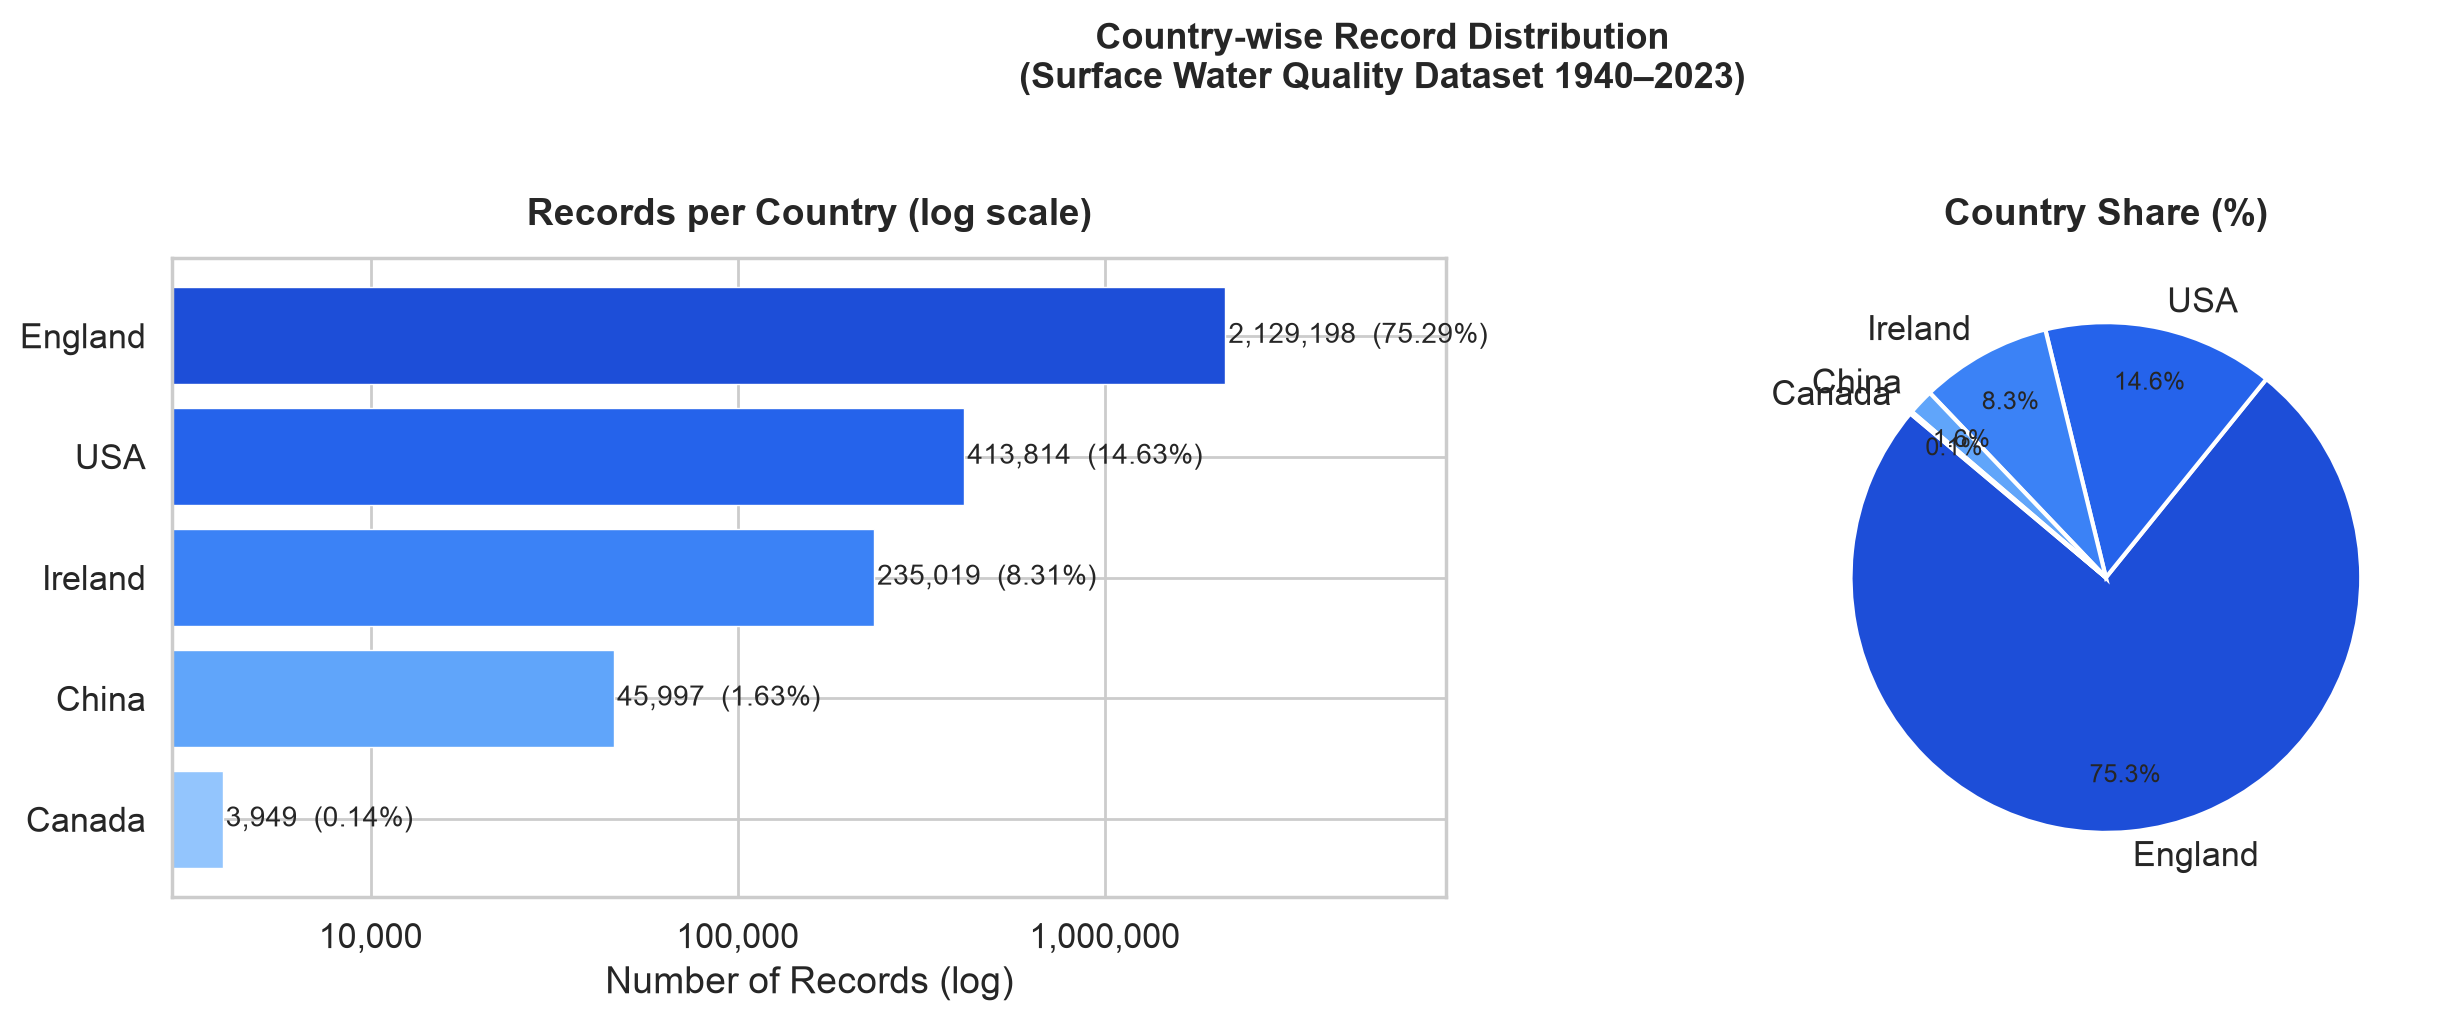
\includegraphics[width=0.95\columnwidth]{figures/01_country_distribution.png}
  \caption{Geographic observation volume across the five monitoring jurisdictions, showing England as the primary telemetry contributor.}
  \label{fig:country_dist}
\end{figure}

\subsection{Thermodynamic Physical Bounds Enforcement}
Sensor telemetry in aquatic environments is susceptible to biological fouling, power supply decay, and transmission dropouts. Grounded in chemical thermodynamics, an axiomatic envelope was enforced (Table~\ref{tab:physics_bounds}). Measurements outside these bounds were identified as telemetry errors and excluded.

\begin{table}[!t]
  \caption{Thermodynamic \& Physical Bounds Screening Envelope}
  \label{tab:physics_bounds}
  \centering
  \setlength{\tabcolsep}{3pt}
  \begin{tabular}{ll>{\raggedright\arraybackslash}p{3.5cm}}
    \toprule
    \textbf{Parameter} & \textbf{Valid Range} & \textbf{Thermodynamic Rationale} \\
    \midrule
    pH & $[3.0,\, 12.0]$ & Acid-base thermodynamic limits \\
    Temp ($T$) & $[0.0,\, 45.0]\,^{\circ}\text{C}$ & Liquid phase boundary for surface waters \\
    DO & $[0.0,\, 25.0]\,\text{mg/L}$ & Henry's law atmospheric ceiling \\
    BOD & $\ge 0.0\,\text{mg/L}$ & Non-negative biological uptake \\
    Ammonia & $\ge 0.0\,\text{mg/L}$ & Non-negative chemical concentration \\
    $\text{PO}_4^{3-}$ & $\ge 0.0\,\text{mg/L}$ & Non-negative chemical concentration \\
    Nitrogen & $\ge 0.0\,\text{mg/L}$ & Non-negative chemical concentration \\
    Nitrate & $\ge 0.0\,\text{mg/L}$ & Non-negative chemical concentration \\
    \bottomrule
  \end{tabular}
\end{table}

\begin{figure}[!t]
  \centering
  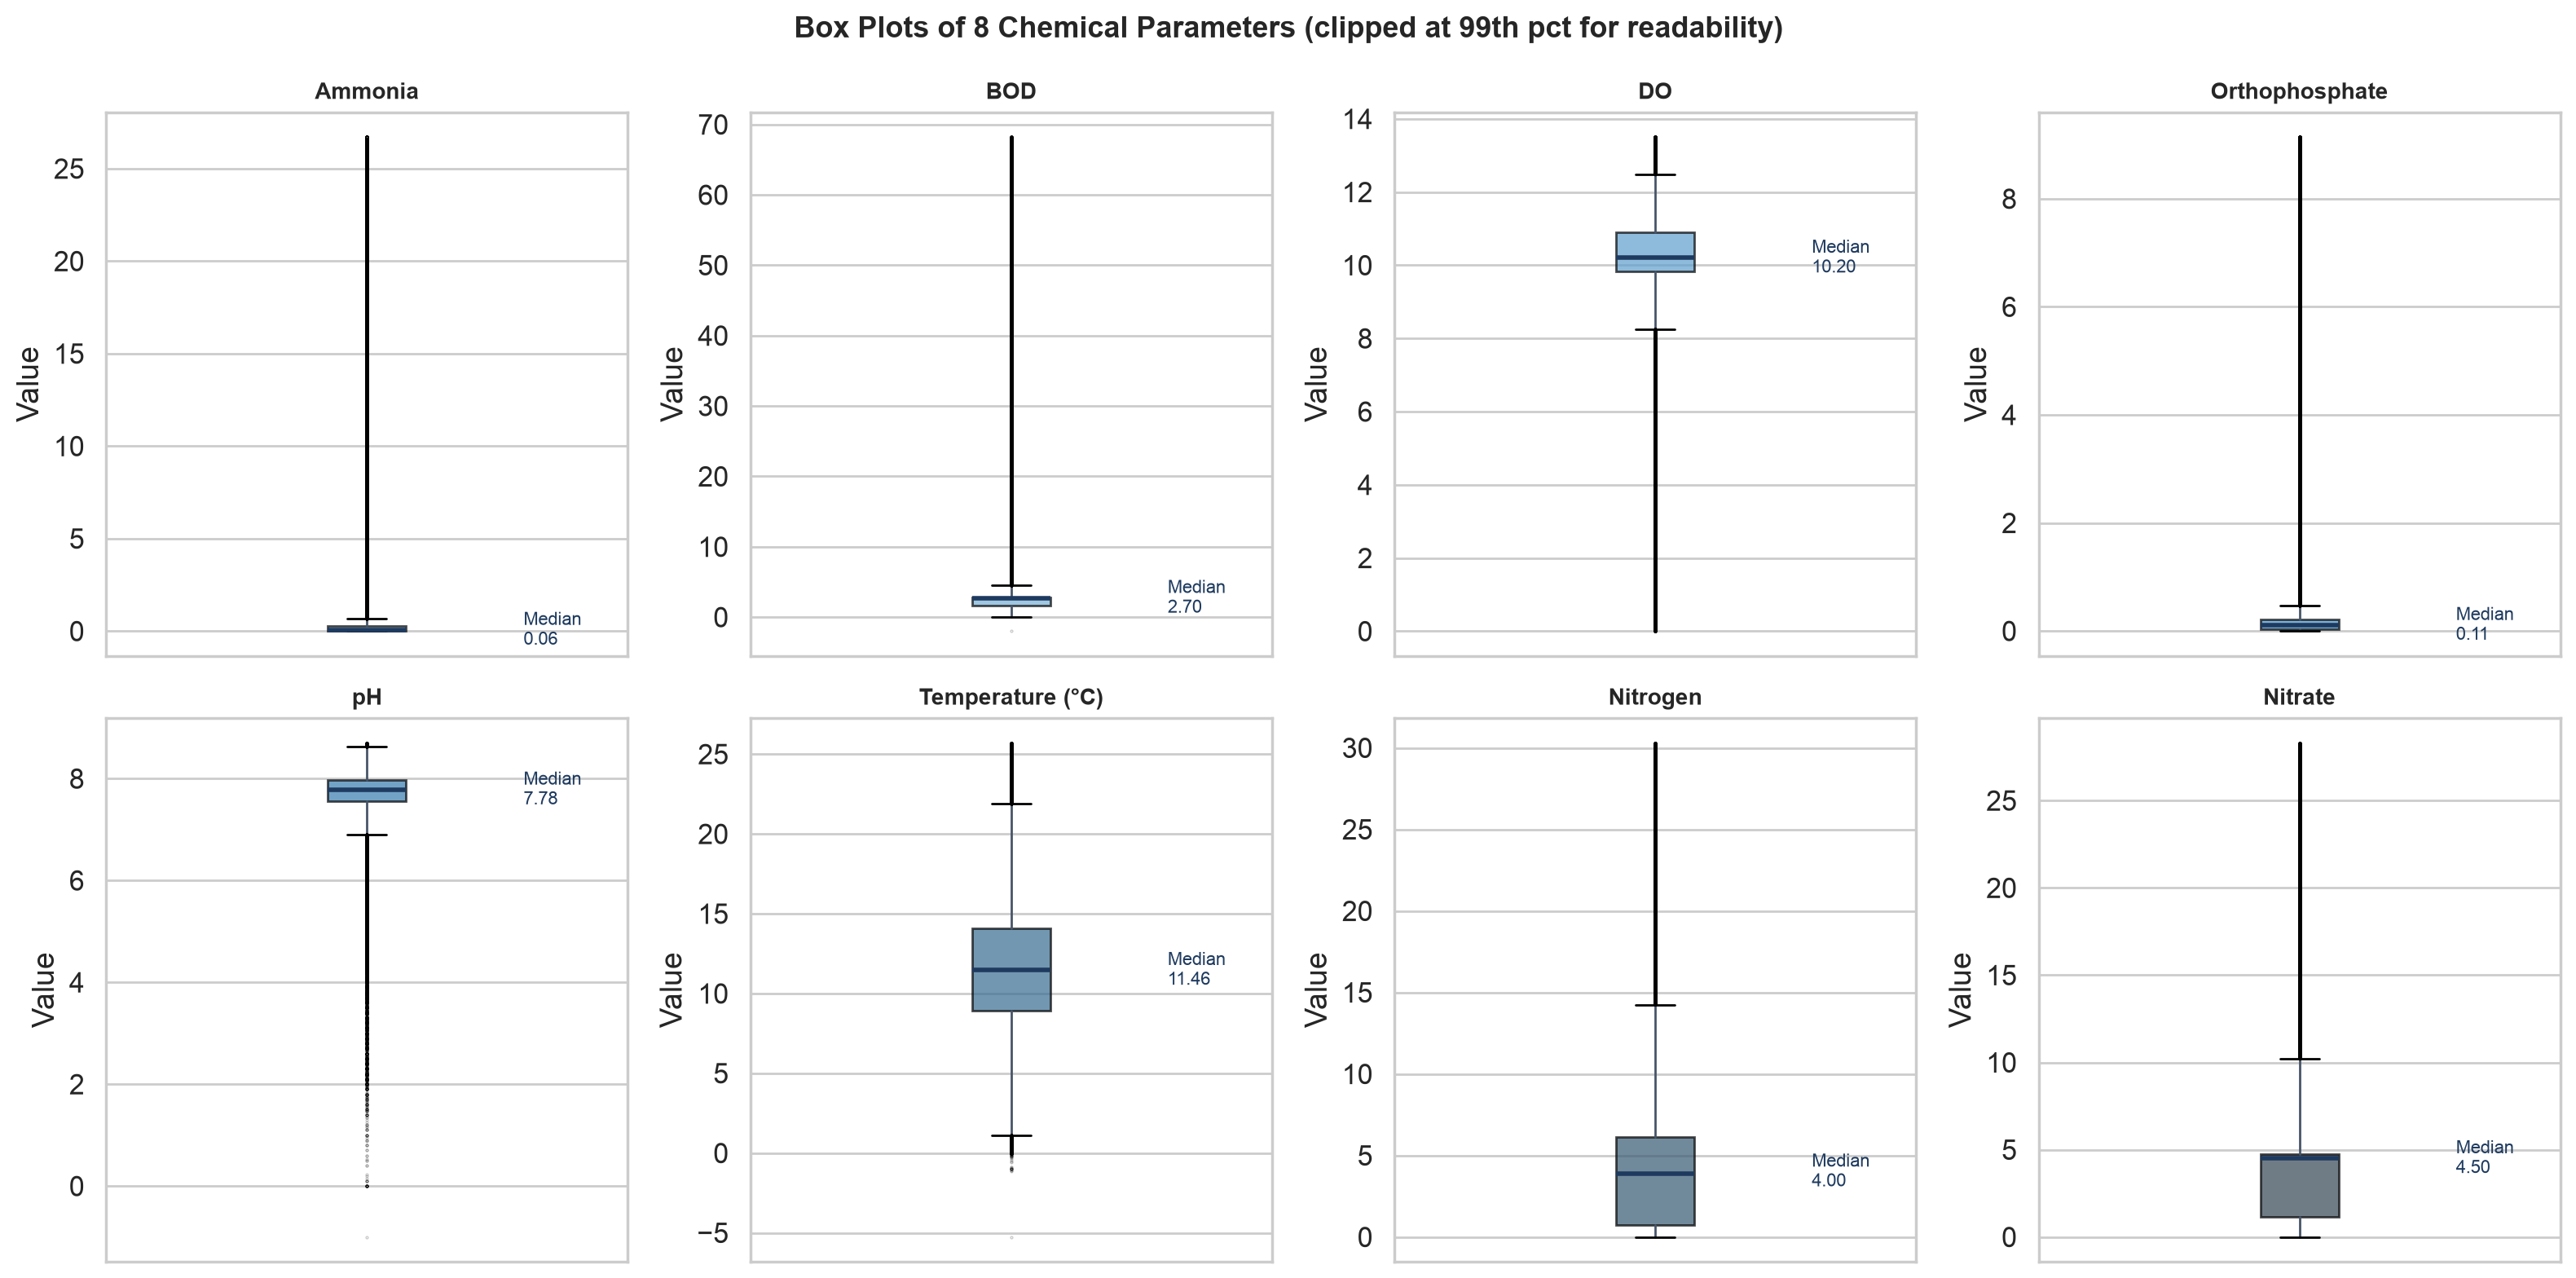
\includegraphics[width=0.95\columnwidth]{figures/04_chemical_boxplots.png}
  \caption{Boxplots demonstrating extreme right-skewness in raw nutrient telemetry (orthophosphate, ammonia, BOD) prior to logarithmic transformation.}
  \label{fig:boxplots}
\end{figure}

\subsection{Target Distribution Analysis}
As depicted in Fig.~\ref{fig:target_dist}, the ground-truth CCME~WQI target displays a characteristic bimodal distribution across the complete-case corpus. The dominant peak at $WQI > 90$ reflects pristine, unpolluted waterways meeting all regulatory compliance criteria ($36.2\%$ of samples reside in the Excellent tier). A secondary distribution spans $WQI \in [35, 75]$, capturing degraded urban and industrial basins experiencing frequent guideline exceedances.

\begin{figure}[!t]
  \centering
  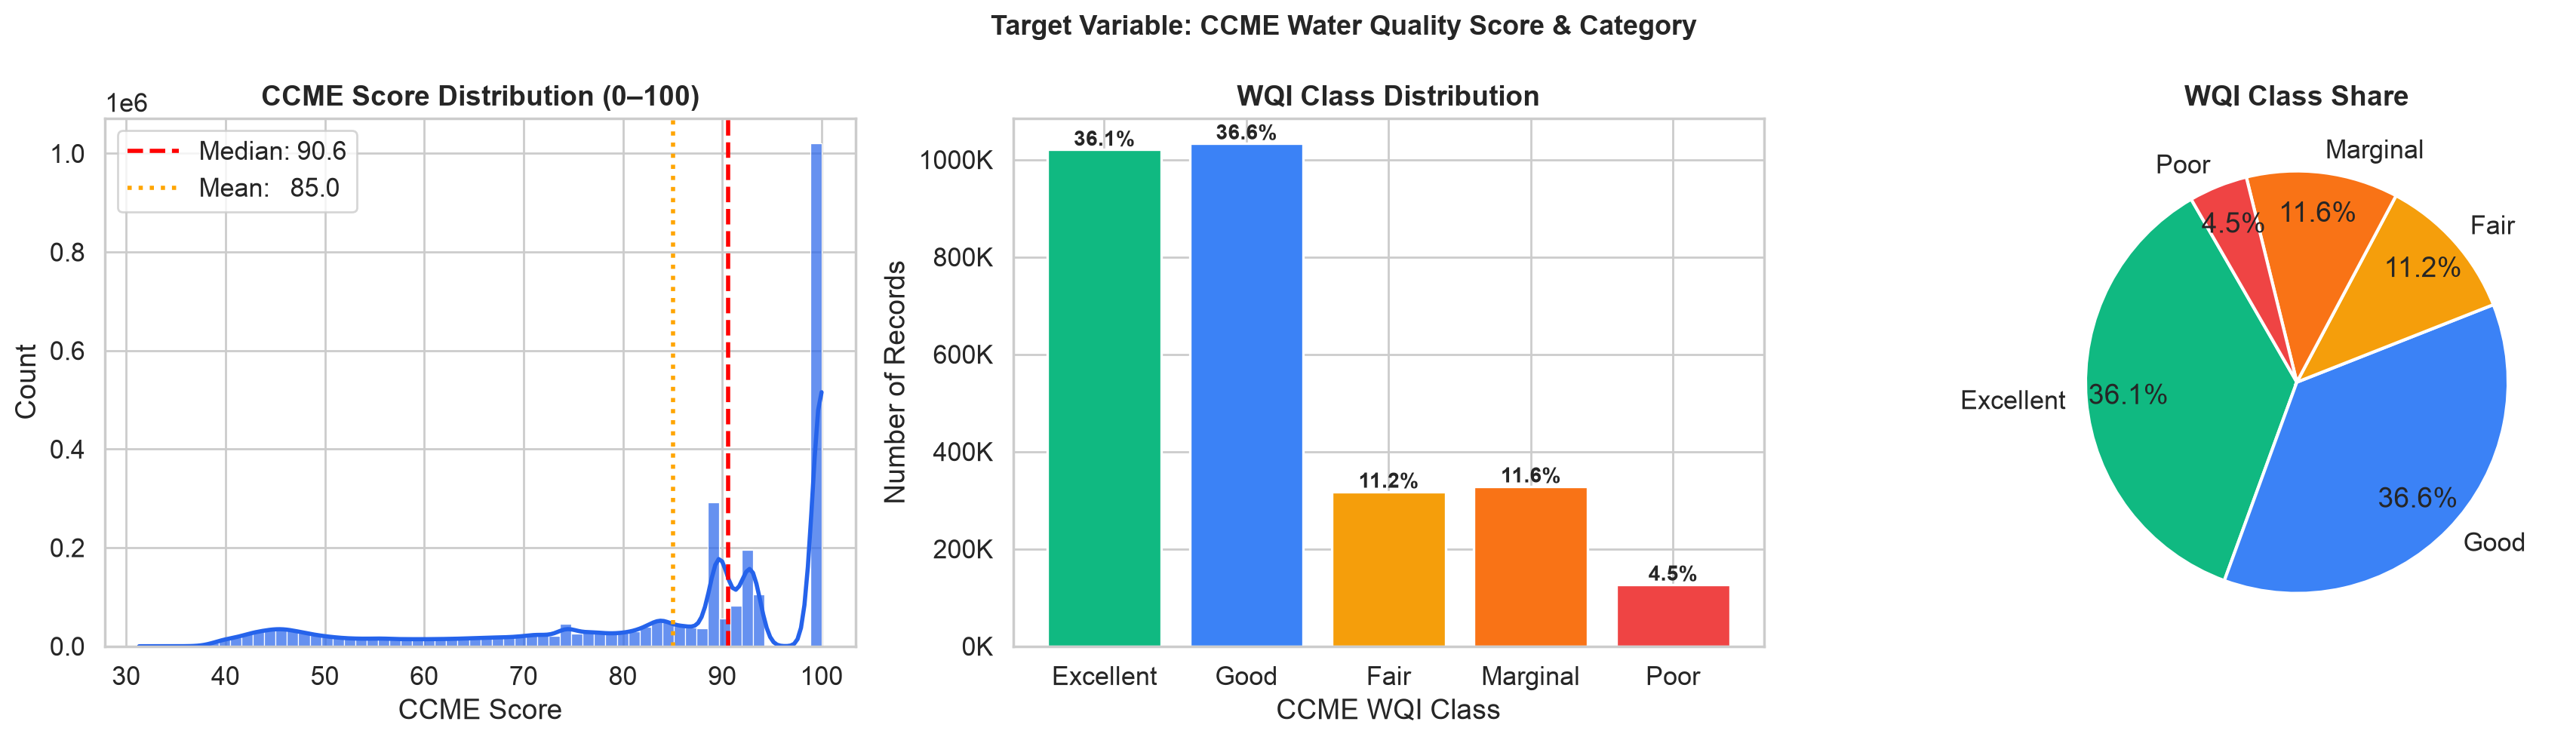
\includegraphics[width=0.95\columnwidth]{figures/11_target_distribution.png}
  \caption{Empirical bimodal distribution of the continuous CCME WQI target ($y \in [0, 100]$) across 2.82 million observations.}
  \label{fig:target_dist}
\end{figure}

% ============================================================
\section{Data Preprocessing \& Feature Engineering}
\label{sec:features}

\subsection{38-Dimensional Tabular Representation (Tree Models)}
Tree-based models rely on an engineered 38-feature representation spanning seven functional categories (Table~\ref{tab:feature_taxonomy}).

\begin{table}[!t]
  \caption{Taxonomy of the 38-Dimensional Tabular Feature Set}
  \label{tab:feature_taxonomy}
  \centering
  \setlength{\tabcolsep}{3pt}
  \begin{tabular}{lp{5.4cm}}
    \toprule
    \textbf{Group (Count)} & \textbf{Constituent Domain Features} \\
    \midrule
    \textbf{Base Telemetry (8)} & pH, Temp ($^{\circ}\text{C}$), DO, BOD, Ammonia, $\text{PO}_4^{3-}$, Total N, $\text{NO}_3^-$ \\
    \textbf{Stoichiometry (7)} & Benson--Krause $\text{DO}_{\%sat}$, DO deficit, Redfield $\text{N}:\text{P}$, Emerson $\text{NH}_{3,\text{toxic}}$, BOD/DO, $\text{NO}_3/\text{N}$, pH neutral dev \\
    \textbf{$\log(1+x)$ Norm (7)} & $\log(1{+}\text{PO}_4)$, $\log(1{+}\text{N})$, $\log(1{+}\text{NH}_4)$, $\log(1{+}\text{BOD})$, $\log(1{+}\text{DO}_{\text{def}})$, $\log(1{+}\text{N:P})$, $\log(1{+}\text{NH}_{3,\text{tox}})$ \\
    \textbf{Station Lags (6)} & Lag-1 shift for DO, Temp, BOD, $\text{PO}_4$, and rolling-3 statistics \\
    \textbf{Stress Counter (1)} & \texttt{exceedance\_counter} (cumulative threshold violations) \\
    \textbf{Contextual (2)} & \texttt{country\_code} (integer), \texttt{waterbody\_type\_code} (integer) \\
    \textbf{Temporal (7)} & Year, Month, Season, Quarter, Day-of-year, $\sin/\cos$ harmonic cycles \\
    \bottomrule
  \end{tabular}
\end{table}

\noindent\textbf{1.\ Benson--Krause Dissolved Oxygen Saturation:}
Atmospheric oxygen solubility in freshwater depends non-linearly on water temperature $T$ ($^{\circ}\text{C}$):
\begin{equation}
  \text{DO}_{\text{sat}} = 14.652 - 0.41022\,T + 0.007991\,T^2 - 0.00007777\,T^3
\end{equation}
\begin{equation}
  \text{DO}_{\%sat} = \frac{\text{DO}}{\text{DO}_{\text{sat}}} \times 100, \quad
  \text{DO}_{\text{def}} = \max(0,\, \text{DO}_{\text{sat}} - \text{DO})
\end{equation}

\noindent\textbf{2.\ Redfield Stoichiometric Ratio:}
The atomic balance of nitrogen to phosphorus governs freshwater eutrophication kinetics:
\begin{equation}
  \text{N:P Ratio} = \frac{\text{Nitrogen (mg/L)}}{\text{Orthophosphate (mg/L)} + 10^{-5}}
\end{equation}

\noindent\textbf{3.\ Emerson Toxic Un-Ionized Ammonia:}
Aqueous ammonia shifts between non-toxic ammonium ($\text{NH}_4^+$) and toxic un-ionized ammonia ($\text{NH}_3$) as a function of temperature and pH:
\begin{equation}
  f_{\text{toxic}} = \frac{1}{10^{(0.09018 + \frac{2729.92}{T+273.15} - \text{pH})} + 1}
\end{equation}
\begin{equation}
  \text{NH}_{3,\text{toxic}} = \text{Ammonia} \times f_{\text{toxic}}
\end{equation}

\begin{figure}[!t]
  \centering
  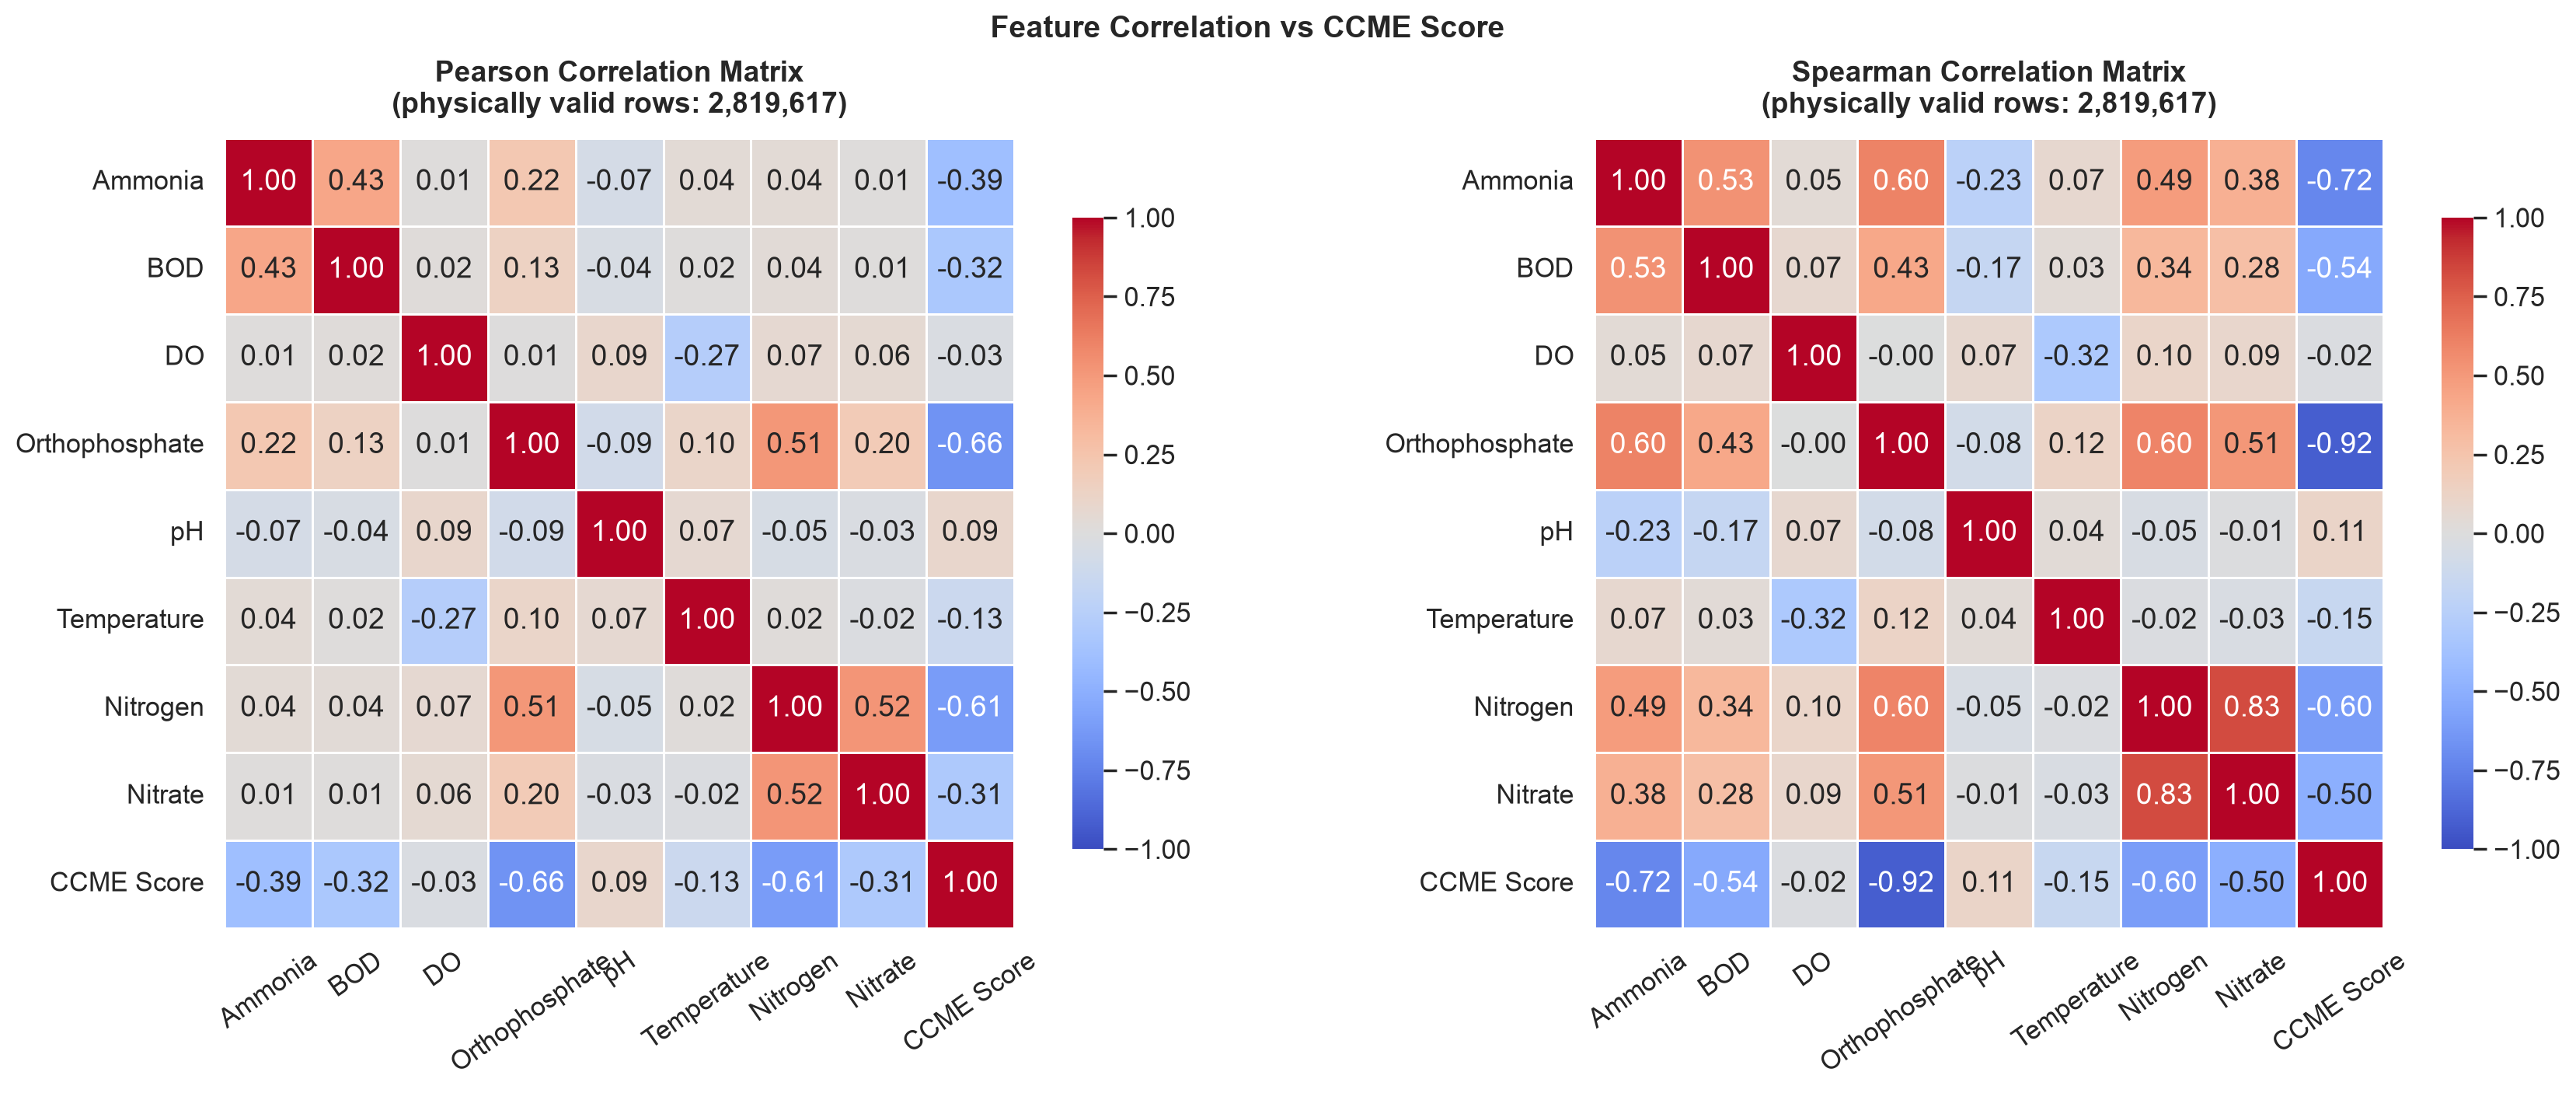
\includegraphics[width=0.95\columnwidth]{figures/08_correlation_heatmaps.png}
  \caption{Pearson correlation matrix across engineered features, showing orthophosphate ($\log(1{+}\text{PO}_4)$) exhibiting the strongest negative correlation with CCME WQI ($r = -0.85$).}
  \label{fig:corr}
\end{figure}

\subsection{53-Dimensional Deep Learning Representation}
Unlike decision trees, neural networks require continuous input conditioning:
\begin{itemize}
  \item \textbf{36 Continuous Features:} Scaled using scikit-learn \texttt{StandardScaler} fit exclusively on the training split.
  \item \textbf{17 Categorical Indicator Features:} One-Hot Encoding of \texttt{country\_code} (5 states) and \texttt{waterbody\_type\_code} (12 habitat classes).
\end{itemize}

\subsection{Anti-Leakage Data Partitioning}
The 2,819,617 cleaned observations were divided using a stratified 70/15/15 protocol:
\begin{itemize}
  \item \textbf{Training Set (70\%):} 1,973,730 observations. Sharded into 5 folds for cross-validation and out-of-fold residual collection.
  \item \textbf{Validation Set (15\%):} 422,944 observations for tuning hyperparameters, learning rate schedules, and early stopping.
  \item \textbf{Held-Out Test Set (15\%):} 422,943 observations quarantined until final frozen benchmark evaluation.
\end{itemize}

% ============================================================
\section{Phase 1: Machine Learning Baselines}
\label{sec:ml}

\subsection{Model Configurations}
\begin{itemize}
  \item \textbf{Mean Baseline Regressor:} Serves as an empirical null benchmark predicting the constant training set mean ($\bar{y} = 86.7233$).
  \item \textbf{Random Forest Regressor:} Bagging ensemble of 30 decision trees, maximum depth 14, minimum samples per leaf 5, and full feature evaluation per split ($m = p$).
  \item \textbf{XGBoost Regressor:} Gradient boosted decision trees with 150 estimators, learning rate $\eta = 0.08$, maximum depth 6, subsample ratio 0.8, column sample by tree 0.8, and histogram-based split finding (\texttt{tree\_method='hist'}).
\end{itemize}

\subsection{Phase 1 Empirical Outcomes}
As depicted in Fig.~\ref{fig:phase1_perf}, both tree ensembles drastically surpass the mean baseline ($\text{MAE} = 14.130$). Random Forest reaches exceptional precision ($\text{MAE} = 0.0514$, $R^2 = 0.99987$), while XGBoost provides high throughput inference ($4.6\text{ ms}$ latency, $\text{MAE} = 0.1614$).

\begin{figure}[!t]
  \centering
  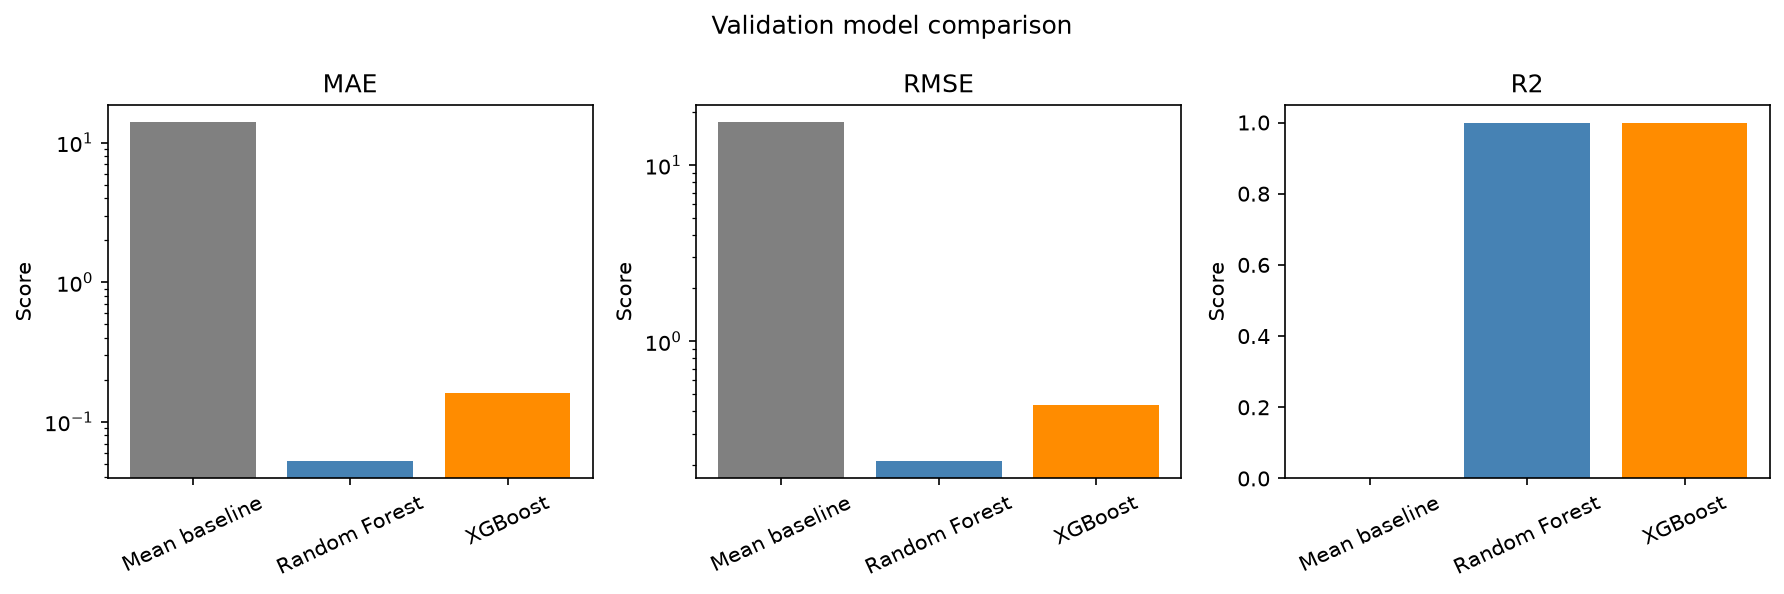
\includegraphics[width=0.95\columnwidth]{figures/14_MODEL_comparison_mae_rmse_r2.png}
  \caption{Phase 1 model performance metrics, demonstrating tree ensemble variance reduction over the empirical mean baseline.}
  \label{fig:phase1_perf}
\end{figure}

\subsection{TreeSHAP Game-Theoretic Attribution}
TreeSHAP attribution on validation data (Fig.~\ref{fig:shap}) reveals that \textbf{orthophosphate accounts for over 88\% of total split importance}. High concentrations drive steep negative Shapley values, aligning with environmental science principles where excess phosphate triggers cyanobacterial blooms and de-oxygenation.

\begin{figure}[!t]
  \centering
  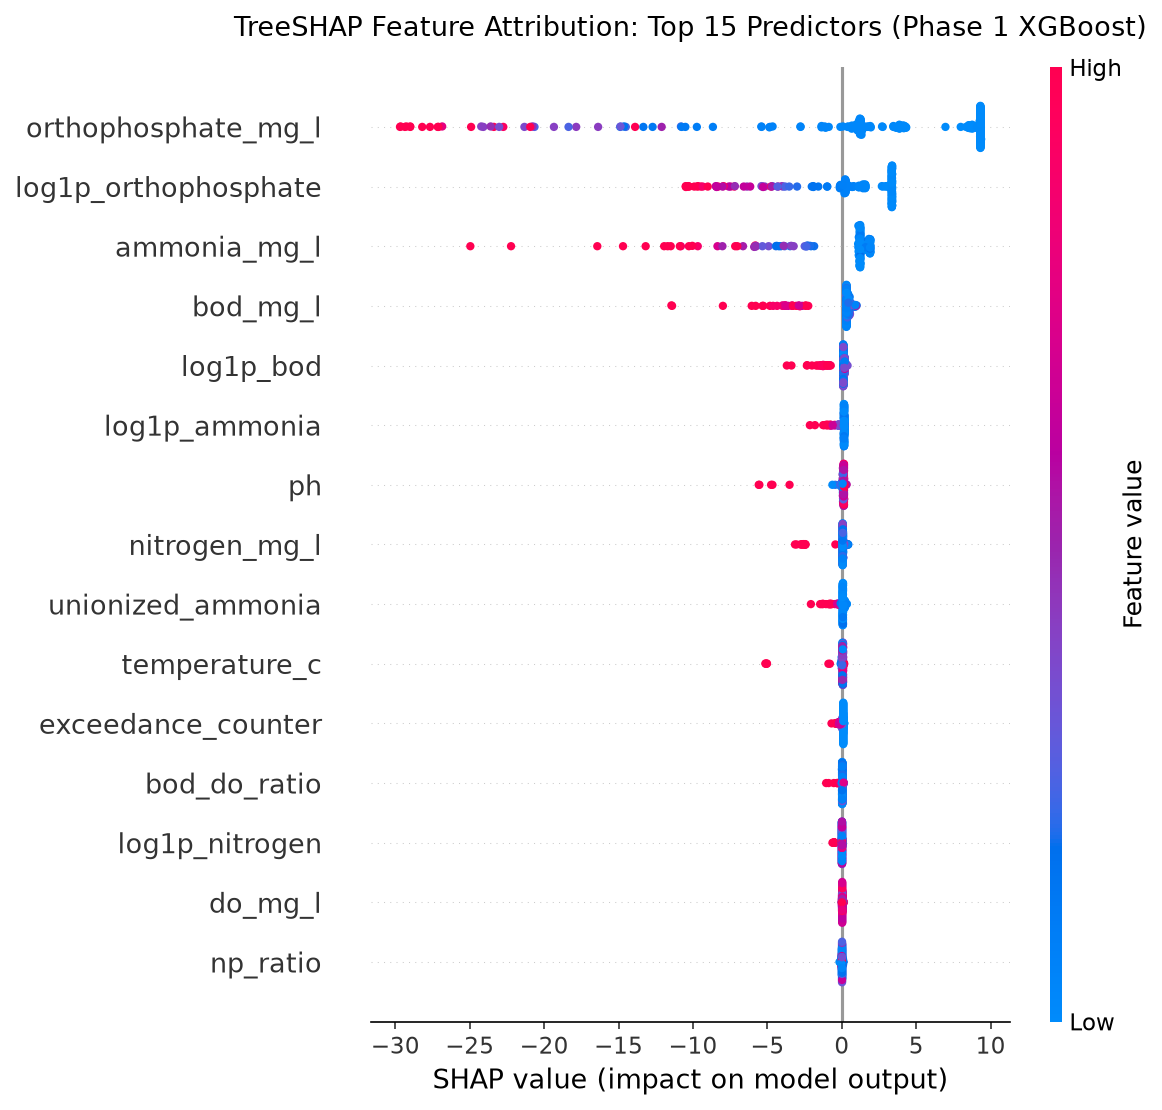
\includegraphics[width=0.95\columnwidth]{figures/16_MODEL_shap_summary_beeswarm.png}
  \caption{TreeSHAP beeswarm attribution plot for Random Forest, illustrating the dominant negative impact of orthophosphate on predicted WQI.}
  \label{fig:shap}
\end{figure}

% ============================================================
\section{Phase 2: Deep Learning Models}
\label{sec:dl}

\subsection{WaterQualityMLP Architecture}
To evaluate neural representation learning on multi-sensor telemetry, we implemented \texttt{WaterQualityMLP} with a 5-layer funnel topology:
\begin{itemize}
  \item \textbf{Input Layer:} 53 dimensions (36 standardized continuous + 17 one-hot categories).
  \item \textbf{Hidden Layers:} Four successive dense blocks: $53 \rightarrow 512 \rightarrow 256 \rightarrow 128 \rightarrow 64 \rightarrow 1$.
  \item \textbf{Regularization \& Normalization:} Each linear projection is followed by \texttt{BatchNorm1d}, ReLU activation, and \texttt{Dropout(p=0.30)}.
  \item \textbf{Initialization:} Kaiming He normal initialization with zero biases.
\end{itemize}

\subsection{Training Loop \& Convergence Diagnostics}
The MLP was optimized using AdamW ($\text{lr} = 10^{-3}$, $\text{weight\_decay} = 10^{-4}$) under Mean Squared Error (MSE) loss with batch size 2,048 over 1,973,730 training samples. Fig.~\ref{fig:mlp_training} illustrates the loss and validation MAE curves across training epochs. The model converged rapidly, attaining its lowest validation loss at epoch 2 ($2.6752$) with a validation MAE of $1.2534$.

\begin{figure}[!t]
  \centering
  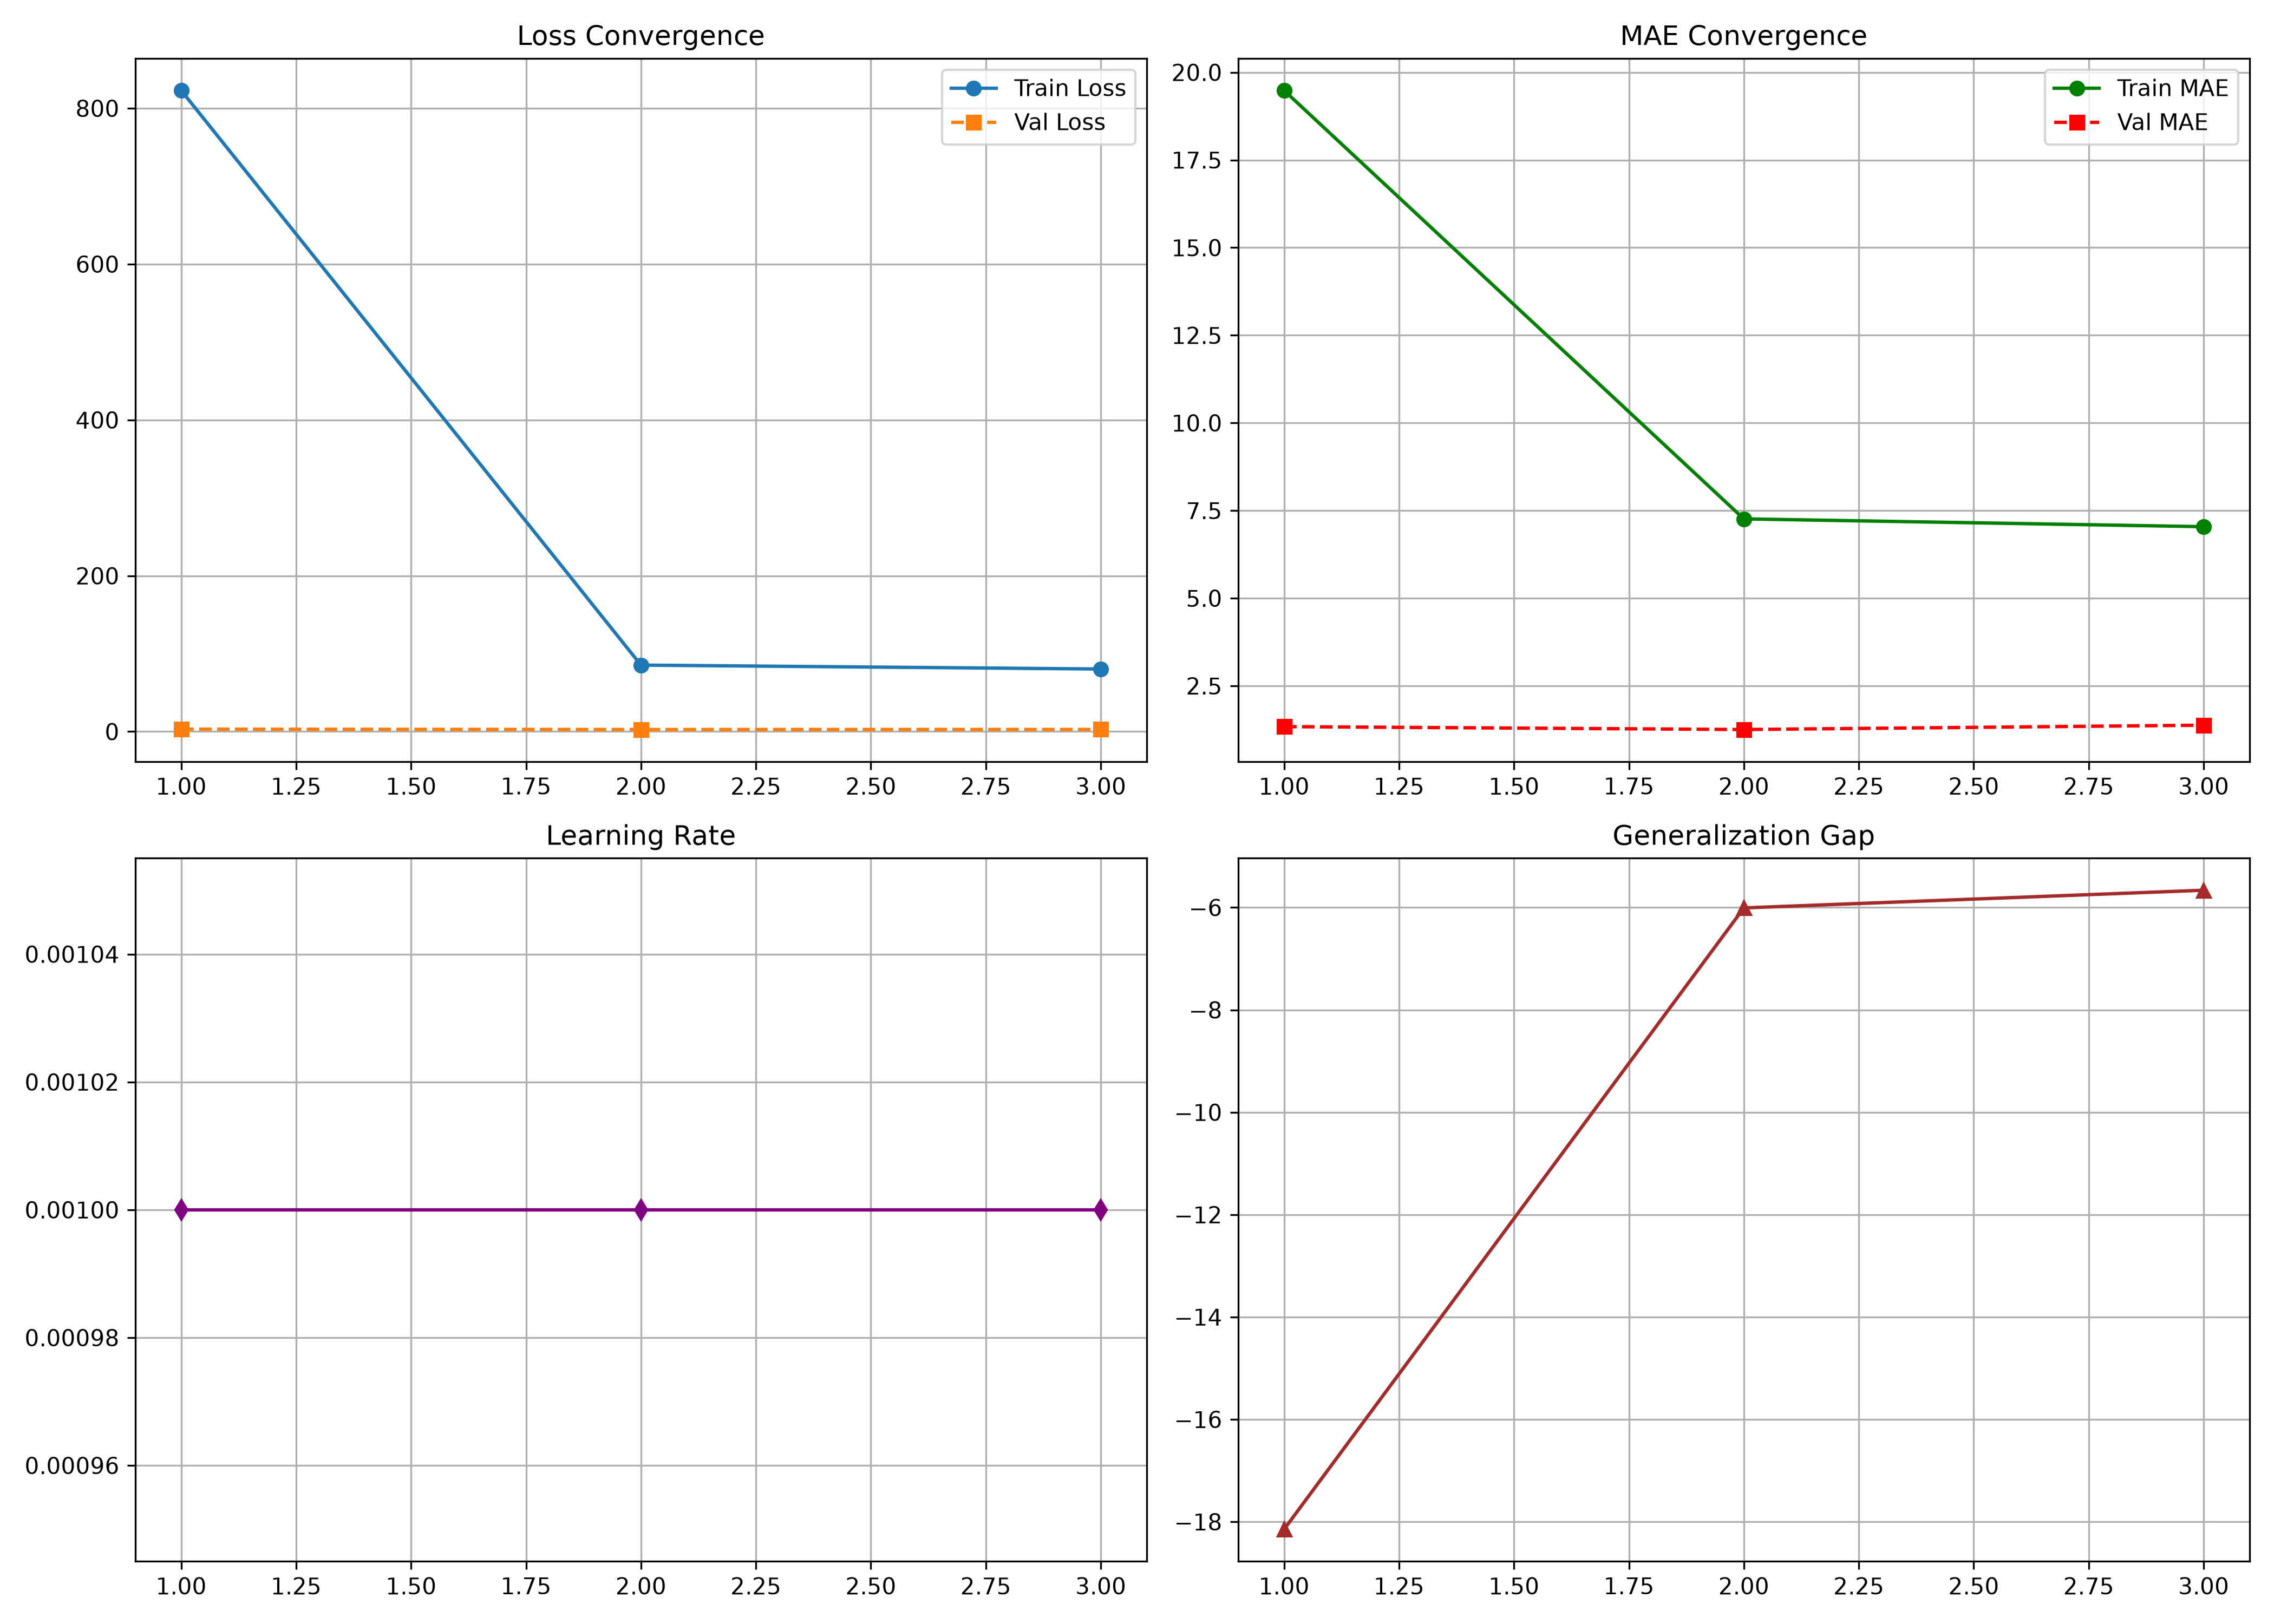
\includegraphics[width=0.95\columnwidth]{figures/03_training_convergence_curves.png}
  \caption{WaterQualityMLP convergence curves across epochs, displaying stable loss reduction and minimal generalization gap under Dropout (0.3).}
  \label{fig:mlp_training}
\end{figure}

On the test set, standalone \texttt{WaterQualityMLP} achieves $\text{MAE} = 1.3800$, $\text{RMSE} = 1.6720$, and $R^2 = 0.99103$. While scientifically respectable, the standalone MLP experiences an order-of-magnitude error gap relative to Random Forest ($\text{MAE} = 0.0514$). This empirical gap illustrates the fundamental challenge of gradient-based optimization on tabular data containing sharp piecewise-constant thresholds.

% ============================================================
\section{Multi-Paradigm Residual Hybrid Architecture}
\label{sec:hybrid}

\subsection{Architectural Motivation \& Formulation}
To unite the orthogonal threshold partitioning of decision trees with the smooth non-linear interpolation of deep neural networks, we designed the \textbf{Residual Hybrid} architecture (Fig.~\ref{fig:hybrid_scatter}).

\begin{figure}[!t]
  \centering
  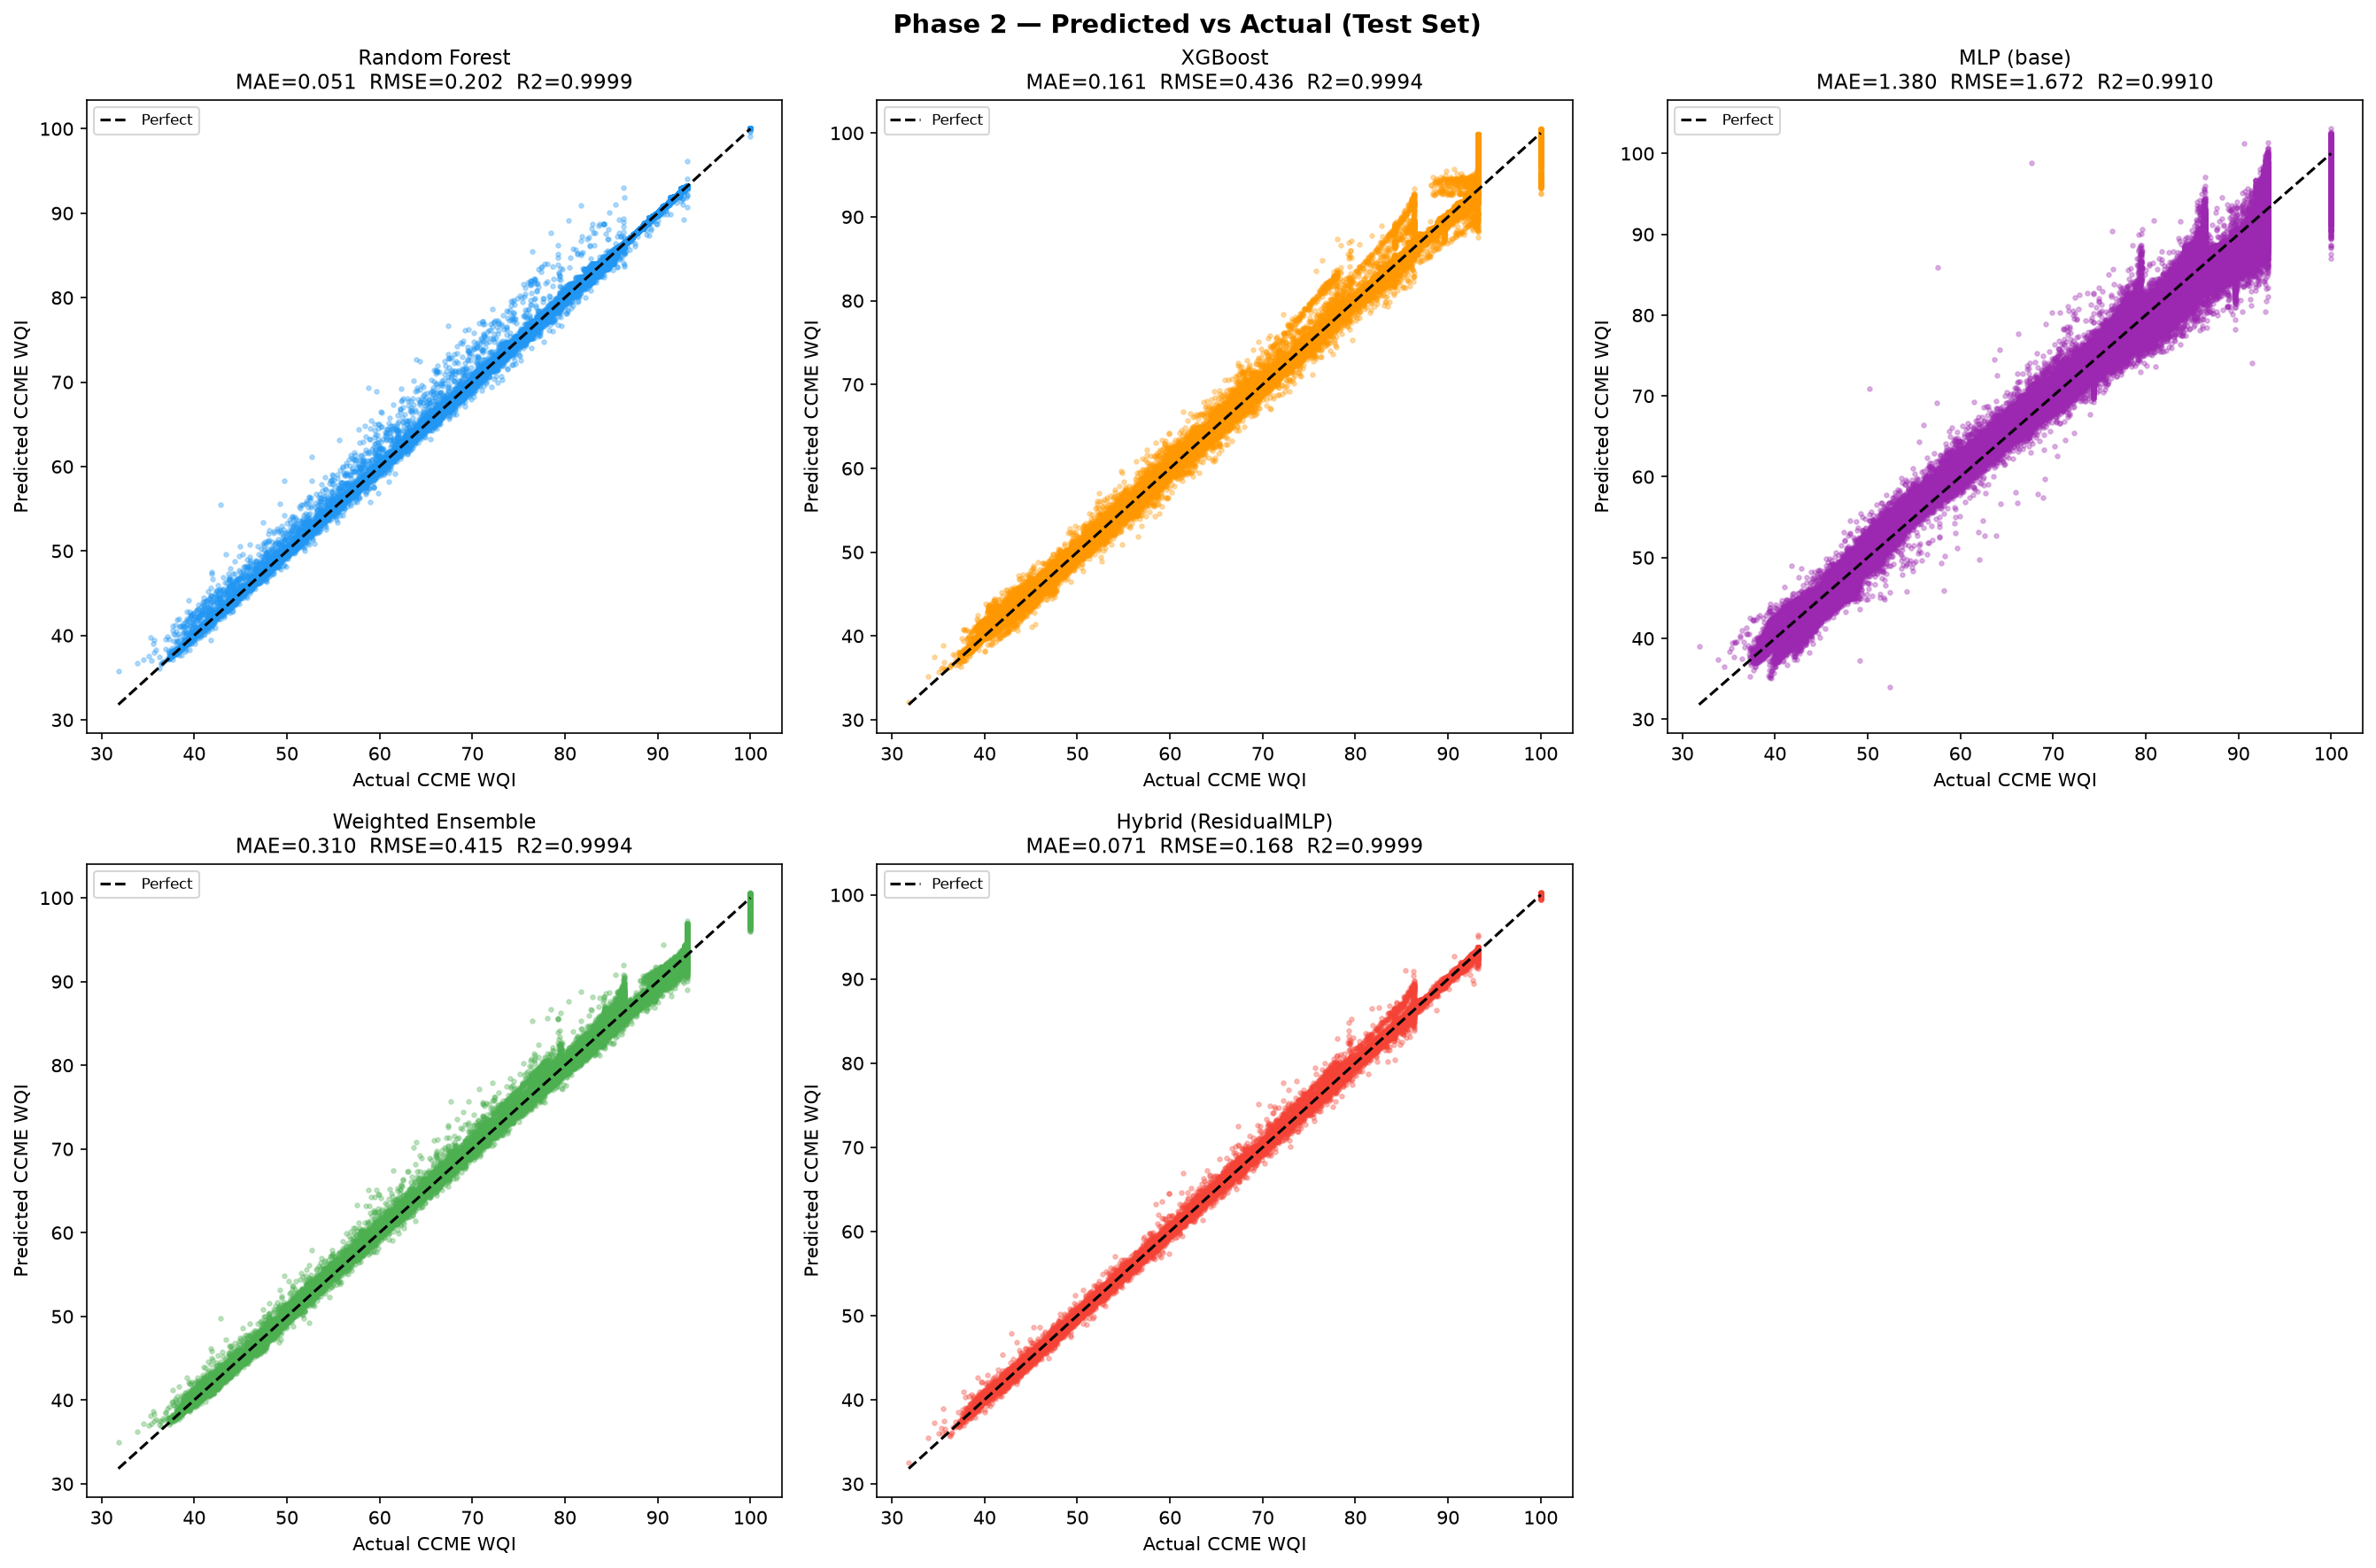
\includegraphics[width=0.95\columnwidth]{figures/hybrid_scatter_plots.png}
  \caption{Scatter plots comparing actual versus predicted values for the Base Tree Ensemble and the Residual Hybrid Model.}
  \label{fig:hybrid_scatter}
\end{figure}

The architecture comprises two stages:
\begin{enumerate}
  \item \textbf{Base Tree Ensemble ($\hat{y}_{\text{base}}$):} An unweighted average of Random Forest and XGBoost predictions:
  \begin{equation}
    \hat{y}_{\text{base}}(x_{\text{tree}}) = 0.5\,\hat{y}_{\text{RF}}(x_{\text{tree}}) + 0.5\,\hat{y}_{\text{XGB}}(x_{\text{tree}})
  \end{equation}
  \item \textbf{Residual Neural Network (\texttt{ResidualMLPNet}):} A 3-hidden-layer MLP that ingests a 54-dimensional feature vector consisting of the 53 deep learning features concatenated with the scalar base tree prediction $\hat{y}_{\text{base}}$:
  \begin{equation}
    x_{\text{res}} = \big[\,x_{\text{DL}} \,\|\, \hat{y}_{\text{base}}\,\big] \in \mathbb{R}^{54}
  \end{equation}
  \begin{equation}
    \hat{r}(x_{\text{res}}) = \text{ResidualMLPNet}(x_{\text{res}})
  \end{equation}
  \item \textbf{Additive Inference:} The final hybrid prediction reconstructs the target:
  \begin{equation}
    \hat{y}_{\text{hybrid}} = \hat{y}_{\text{base}}(x_{\text{tree}}) + \hat{r}(x_{\text{res}})
  \end{equation}
\end{enumerate}

To train the residual network without target contamination:
\begin{itemize}
  \item The training split was partitioned into 5 stratified folds.
  \item For each fold $k \in \{1,\dots,5\}$, base trees were fit on folds $j \neq k$ and evaluated on fold $k$.
  \item Unbiased OOF residual targets were recorded:
  \begin{equation}
    r_i = y_i - \hat{y}_{\text{base}}^{\text{OOF}}(x_i)
  \end{equation}
  \item \texttt{ResidualMLPNet} was trained on these OOF residuals using Smooth L1 loss ($\beta = 1.0$), ensuring zero data leakage into the test set.
\end{itemize}

\begin{figure}[!t]
  \centering
  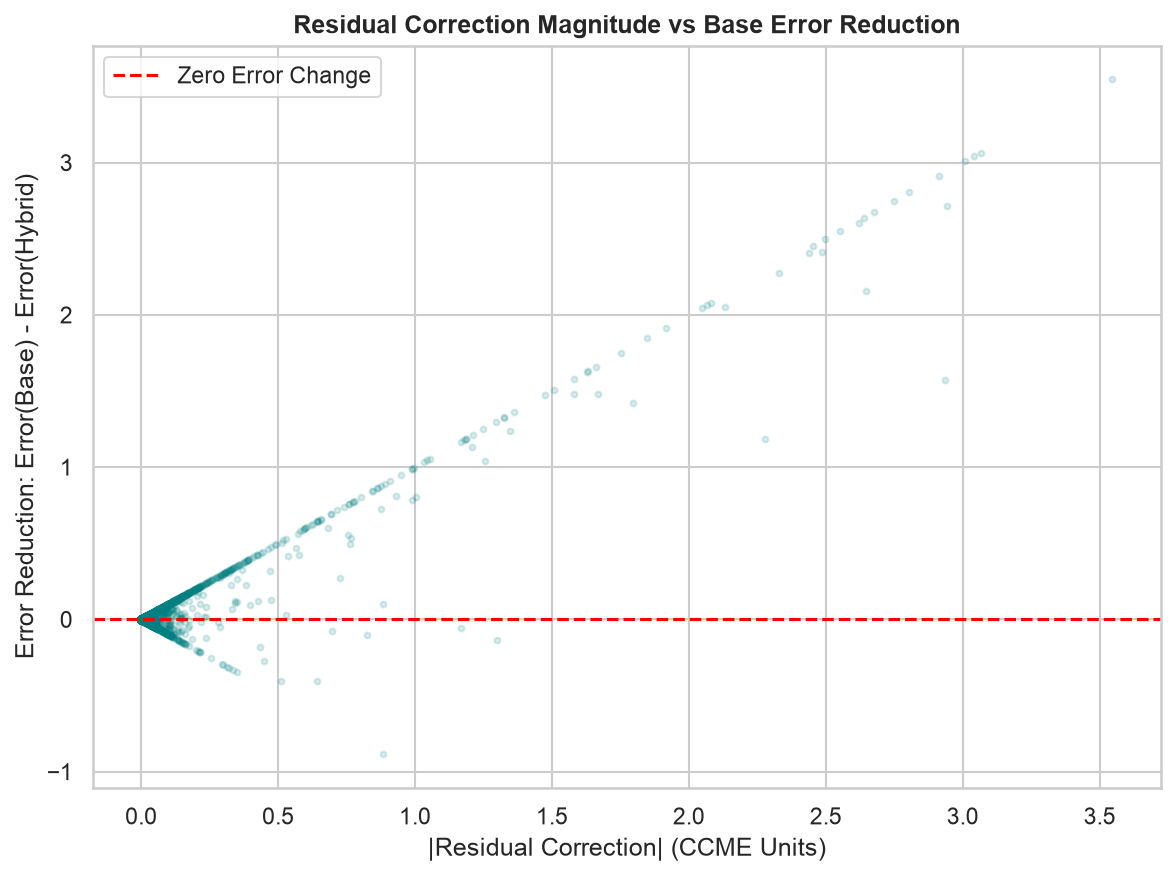
\includegraphics[width=0.95\columnwidth]{figures/correction_vs_base_error.png}
  \caption{Empirical correlation ($r = 0.5262$) between the base tree prediction error and the neural residual correction, proving targeted error correction.}
  \label{fig:correction_vs_error}
\end{figure}

Fig.~\ref{fig:correction_vs_error} plots the neural residual correction $\hat{r}$ against the actual error committed by the base tree ensemble. The strong positive correlation ($r = 0.5262$) demonstrates that the neural network specifically activates when the tree ensemble makes substantial prediction errors.

% ============================================================
\section{Experimental Results \& Comparative Benchmarking}
\label{sec:results}

\subsection{Comprehensive 6-Model Benchmark}
Table~\ref{tab:master_benchmark} presents the comprehensive evaluation of all six predictive paradigms on the common held-out test split of 422,943 observations.

\begin{table*}[!t]
  \caption{Unified Model Performance Benchmark on Common Held-Out Test Set ($N = 422,943$ Records)}
  \label{tab:master_benchmark}
  \centering
  \setlength{\tabcolsep}{5pt}
  \begin{tabular}{llccrrrrrr}
    \toprule
    \textbf{Rank} & \textbf{Model Architecture} & \textbf{Paradigm} & \textbf{Input Dim} & \textbf{MAE} & \textbf{RMSE} & \textbf{$R^2$} & \textbf{MedAE} & \textbf{Max AE} & \textbf{Single Latency} \\
    \midrule
    \textbf{1} & \textbf{Random Forest}      & Bagging Trees       & 38 Tabular          & \textbf{0.0514} & 0.2016          & 0.999870          & \textbf{0.0042} & 12.6128          & $18.2\text{ ms}$ \\
    \textbf{2} & \textbf{Residual Hybrid}   & Tree + Residual MLP & 38 Tab + 53 DL      & 0.0710          & \textbf{0.1678} & \textbf{0.999910} & 0.0229          & \textbf{5.6842}  & $32.4\text{ ms}$ \\
    \textbf{3} & \textbf{Base Tree Ensemble} & Equal Trees (50/50) & 38 Tabular          & 0.0900          & 0.2464          & 0.999805          & 0.0261          & 8.7128           & $22.8\text{ ms}$ \\
    \textbf{4} & \textbf{XGBoost}            & Gradient Boosting   & 38 Tabular          & 0.1614          & 0.4364          & 0.999389          & 0.0480          & 9.2769           & \textbf{4.6\,ms} \\
    \textbf{5} & \textbf{Weighted Ensemble}  & Convex Linear Blend & 38 Tab + 53 DL      & 0.3096          & 0.4155          & 0.999446          & 0.2653          & 8.8283           & $36.1\text{ ms}$ \\
    \textbf{6} & \textbf{WaterQualityMLP}    & Deep Neural Net     & 53 (36 num+17 OHE)  & 1.3800          & 1.6720          & 0.991029          & 1.2893          & 31.1327          & $14.3\text{ ms}$ \\
    \bottomrule
  \end{tabular}
\end{table*}

\begin{figure}[!t]
  \centering
  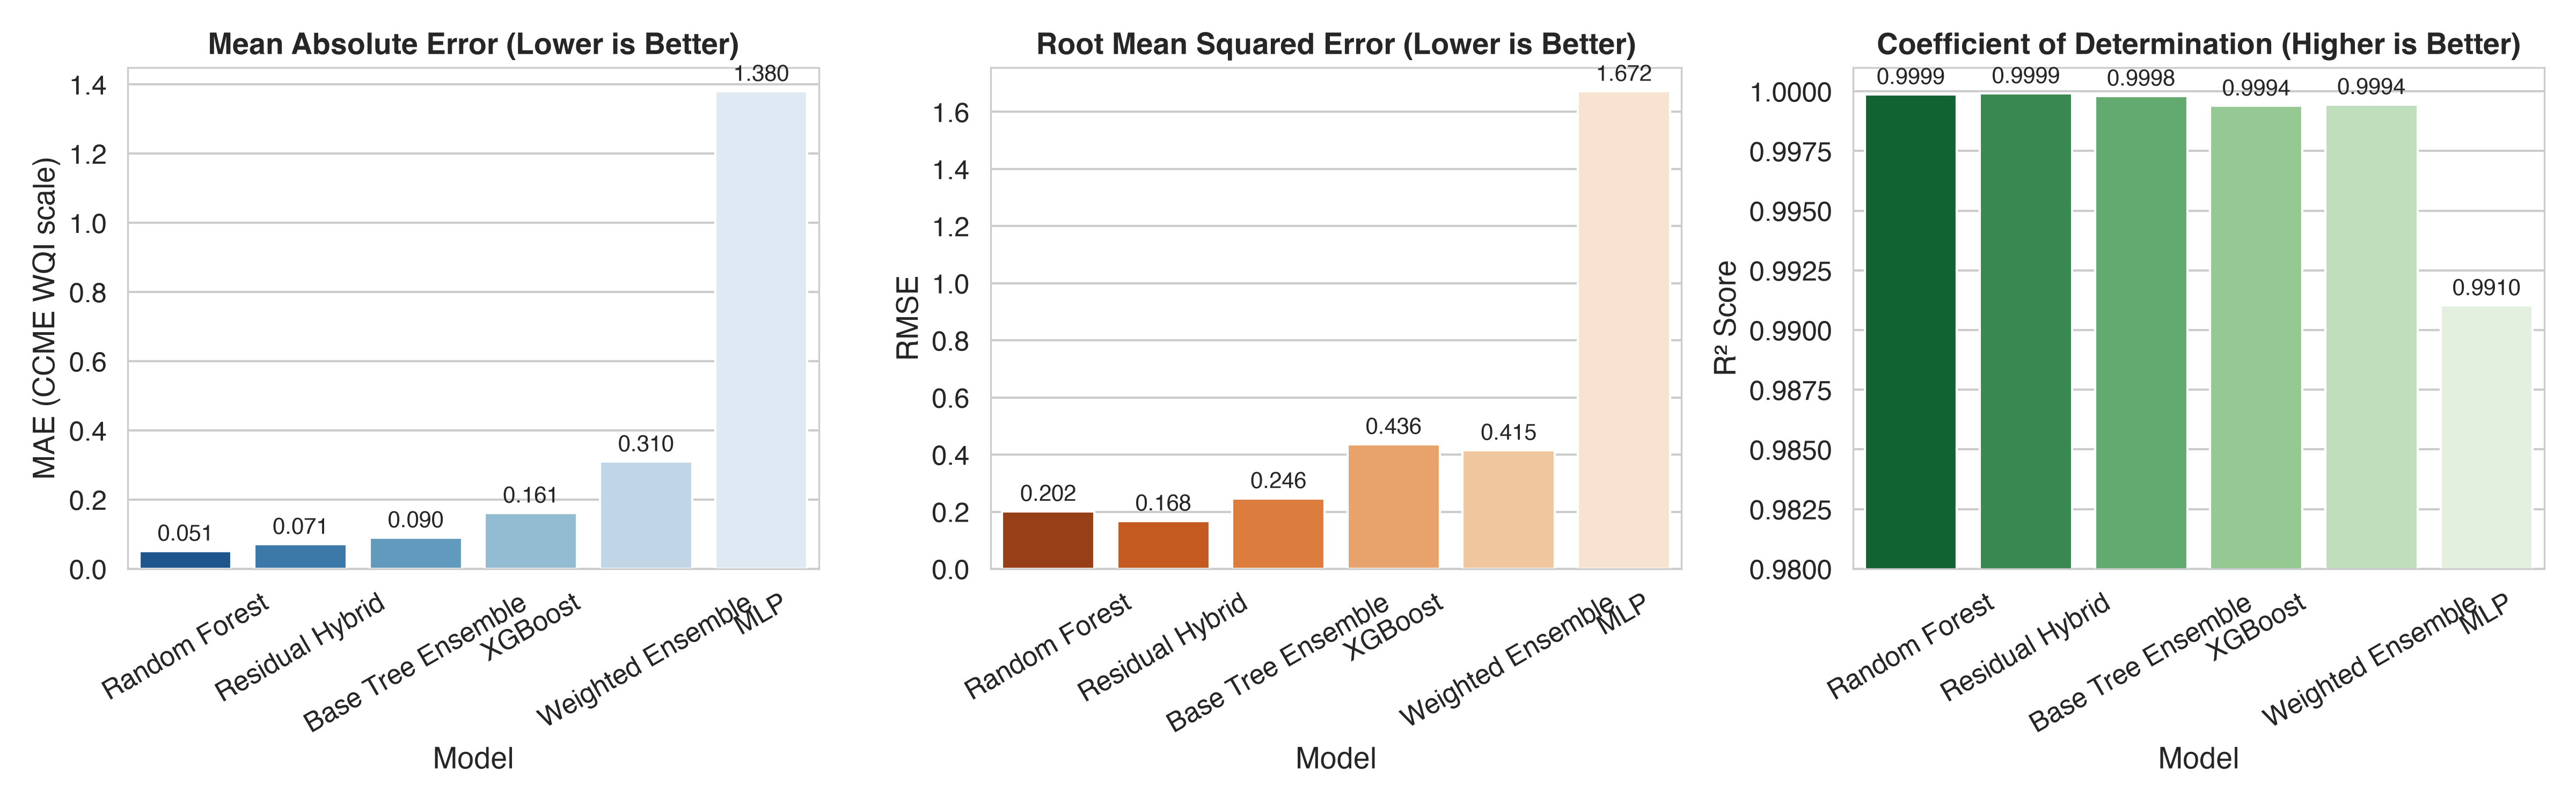
\includegraphics[width=0.95\columnwidth]{figures/model_performance_comparison.png}
  \caption{Unified 6-model benchmark on the held-out test set comparing MAE, RMSE, and $R^2$.}
  \label{fig:model_perf}
\end{figure}

\begin{figure}[!t]
  \centering
  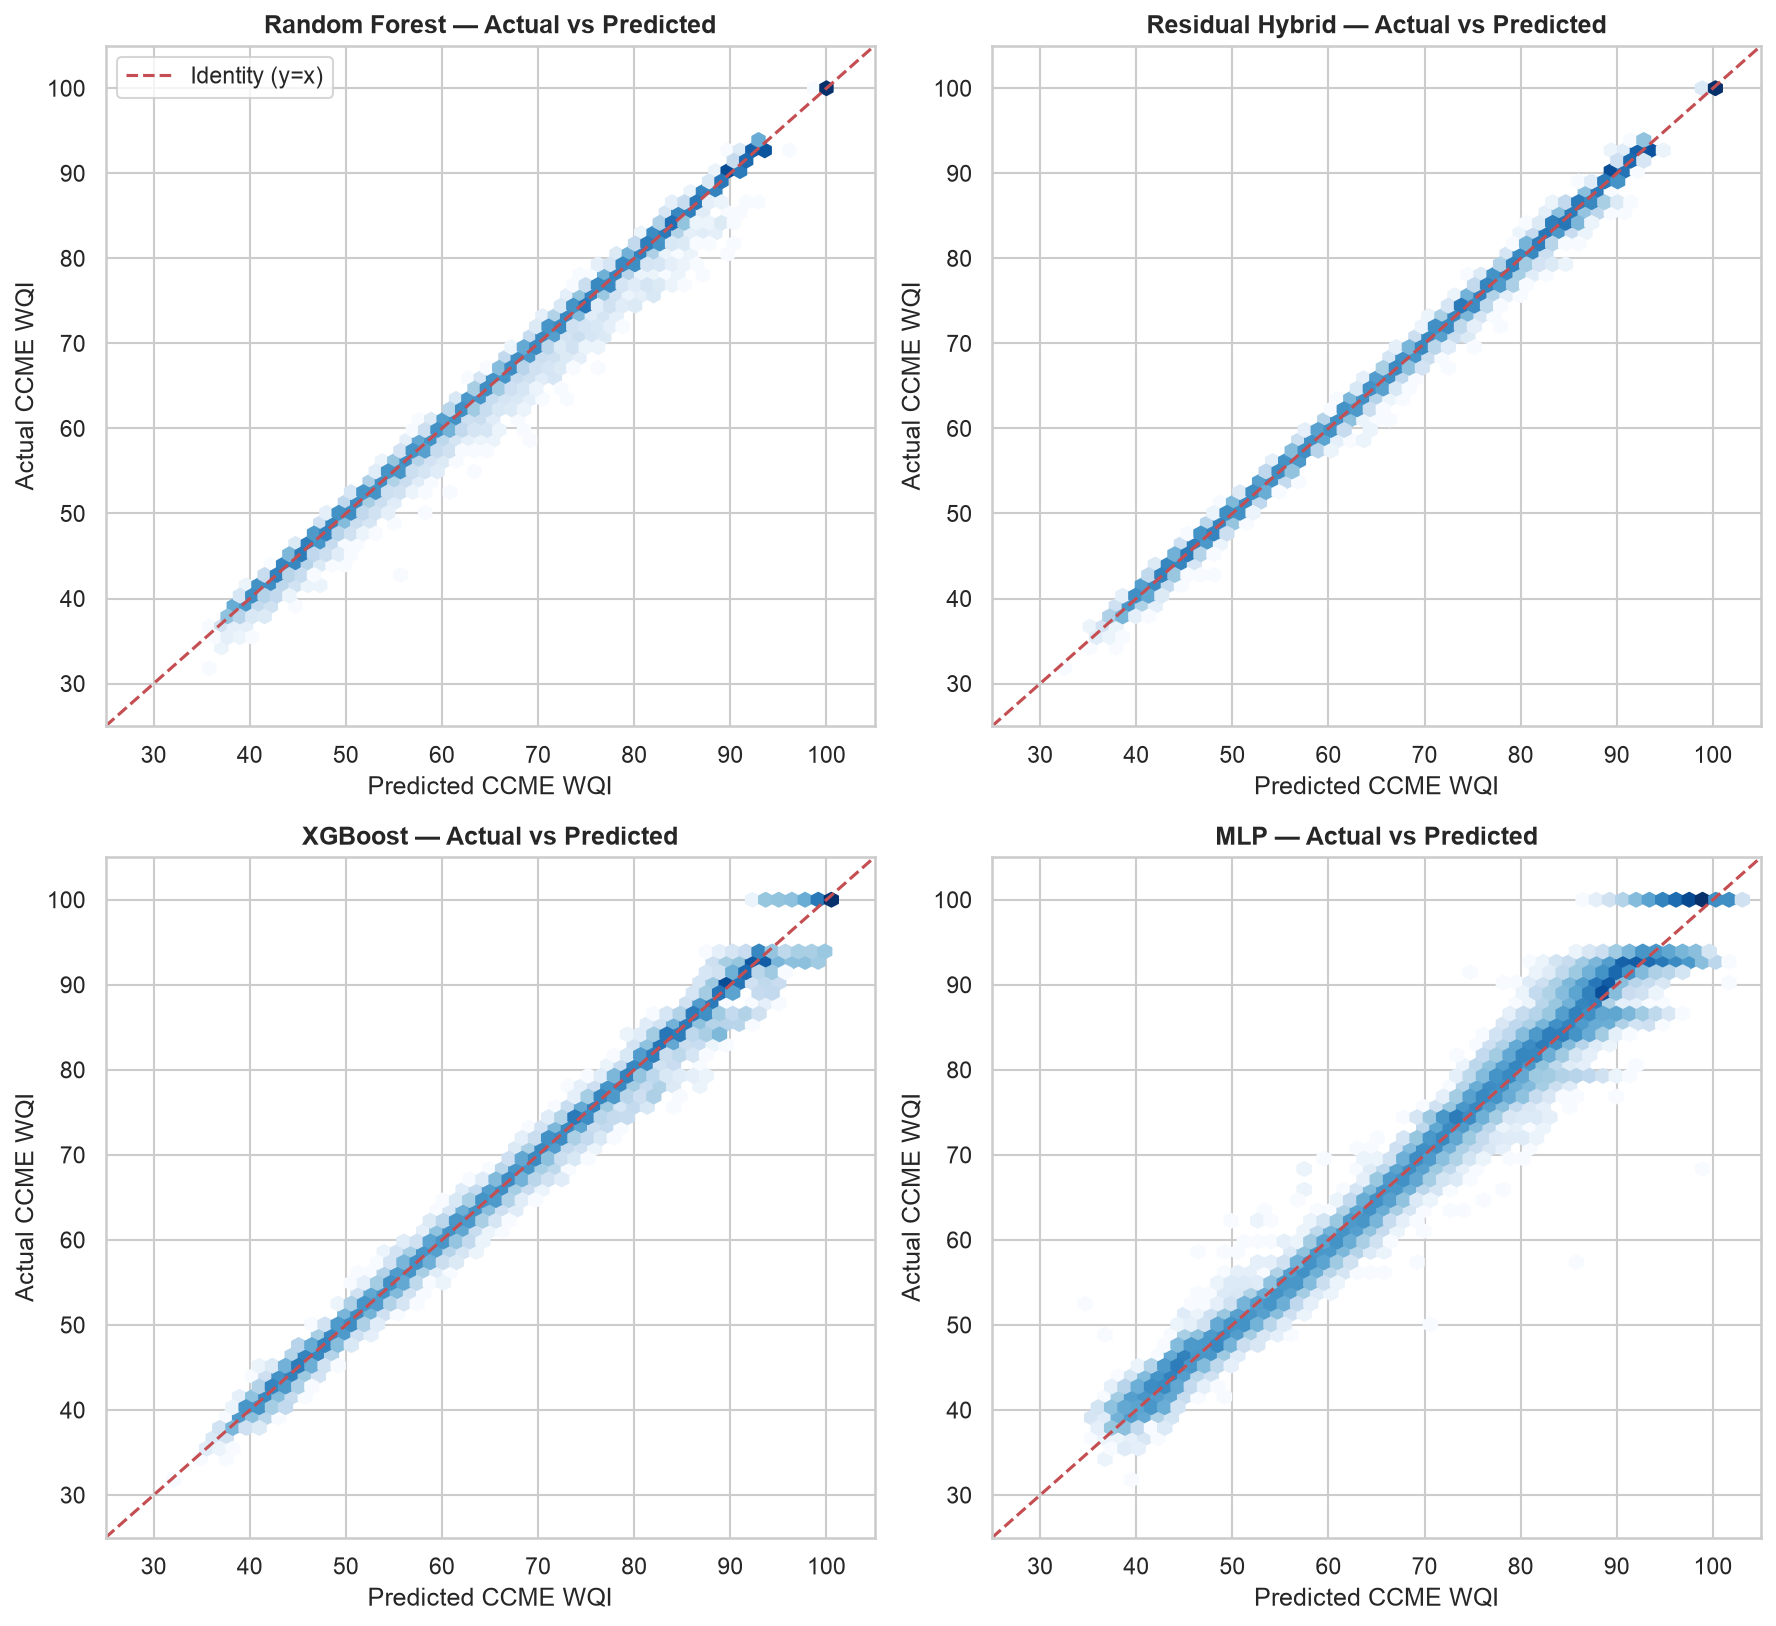
\includegraphics[width=0.95\columnwidth]{figures/actual_vs_predicted.png}
  \caption{Actual versus predicted CCME WQI scatter plots on the test partition, demonstrating the tight identity diagonal across tree and hybrid models.}
  \label{fig:actual_vs_pred}
\end{figure}

\subsection{Key Scientific Trade-Offs}
\noindent\textbf{1.\ Peak Outlier Error Compression:}
Random Forest achieves the lowest median error across typical water quality regimes, but produces severe errors on rare, extreme chemical spikes ($\text{Max AE} = 12.6128$). The Residual Hybrid compresses the worst-case prediction error to \textbf{$5.6842$}, representing a \textbf{$54.9\%$ peak error reduction}.

\noindent\textbf{2.\ Global Variance Minimization:}
Because RMSE heavily penalizes large errors, the Residual Hybrid attains the lowest global RMSE across all architectures (\textbf{$0.1678$}, representing a \textbf{$31.9\%$ variance reduction} over the Base Tree Ensemble).

\noindent\textbf{3.\ Cumulative Error Distribution:}
Fig.~\ref{fig:cdf} plots the Cumulative Distribution Function (CDF) of absolute errors. Over $95\%$ of Residual Hybrid predictions exhibit absolute error below $0.2039$ index units.

\begin{figure}[!t]
  \centering
  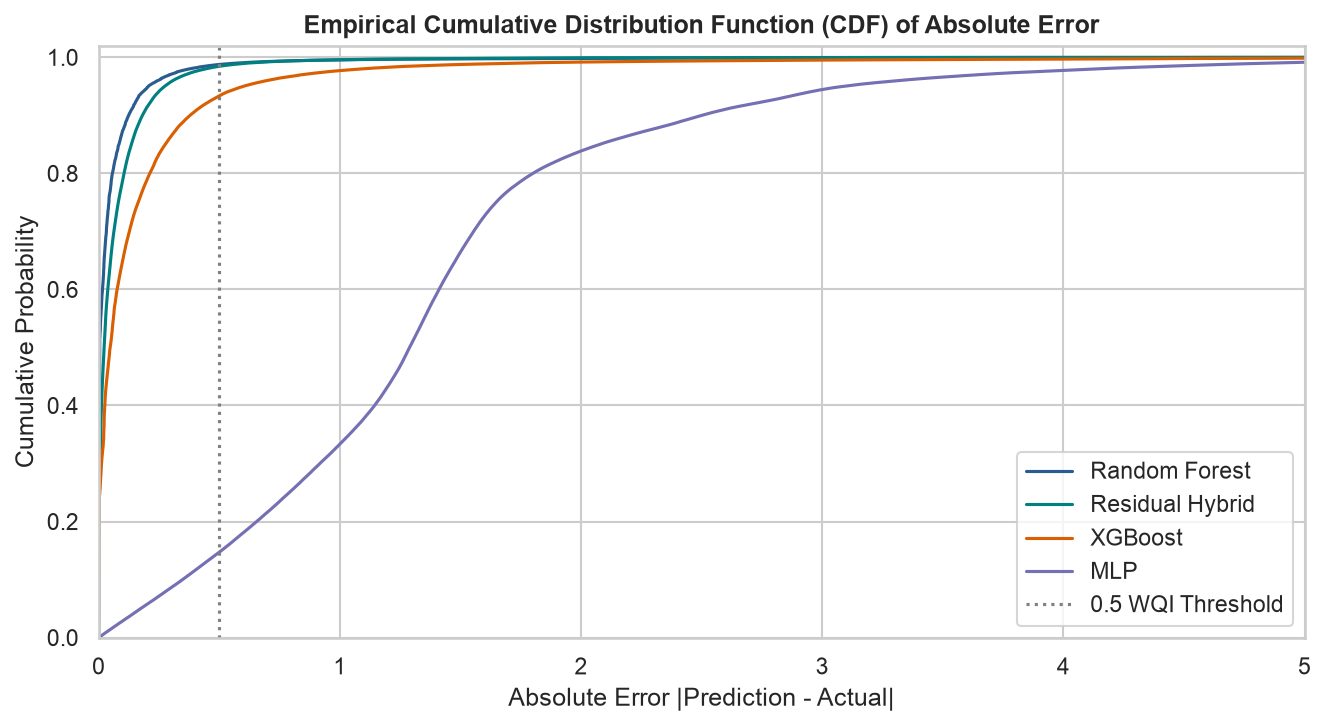
\includegraphics[width=0.95\columnwidth]{figures/absolute_error_cdf.png}
  \caption{Cumulative Distribution Function (CDF) of absolute prediction errors across models on the held-out test split.}
  \label{fig:cdf}
\end{figure}

% ============================================================
\section{Ablation, Regularization \& Computational Profiling}
\label{sec:ablation}

\subsection{7-Group Feature Ablation Analysis}
To quantify the marginal information contribution of each domain subsystem, a Leave-One-Group-Out (LOGO) ablation protocol was conducted on 50,000 validation samples (Table~\ref{tab:ablation_results} and Fig.~\ref{fig:ablation}).

\begin{table}[!t]
  \caption{7-Group Leave-One-Group-Out (LOGO) Feature Ablation Impact}
  \label{tab:ablation_results}
  \centering
  \setlength{\tabcolsep}{3pt}
  \begin{tabular}{lrrrr}
    \toprule
    \textbf{Ablated Group} & \textbf{Feats} & \textbf{RF $\Delta\text{MAE}$} & \textbf{XGB $\Delta\text{MAE}$} & \textbf{MLP $\Delta\text{MAE}$} \\
    \midrule
    \textbf{Baseline (Full)} & 0 & 0.0000 & 0.0000 & 0.0000 \\
    \textbf{\texttt{base\_sensors}} & 8 & \textbf{+12.5749} & \textbf{+21.6473} & +0.4090 \\
    \textbf{\texttt{log1p\_norm}}   & 7 & +7.8952 & +1.6068 & \textbf{+12.1642} \\
    \textbf{\texttt{stoichiometry}} & 7 & +0.0183 & +1.1525 & +0.0363 \\
    \textbf{\texttt{env\_stress}}   & 1 & +0.0000 & +0.1952 & +0.5474 \\
    \textbf{\texttt{contextual}}    & 2 & +0.0000 & +0.0009 & +0.4214 \\
    \textbf{\texttt{history\_lags}} & 6 & -0.0000 & +0.0406 & +0.0139 \\
    \textbf{\texttt{temporal}}      & 7 & -0.0001 & +0.0002 & +0.0299 \\
    \bottomrule
  \end{tabular}
\end{table}

\begin{figure}[!t]
  \centering
  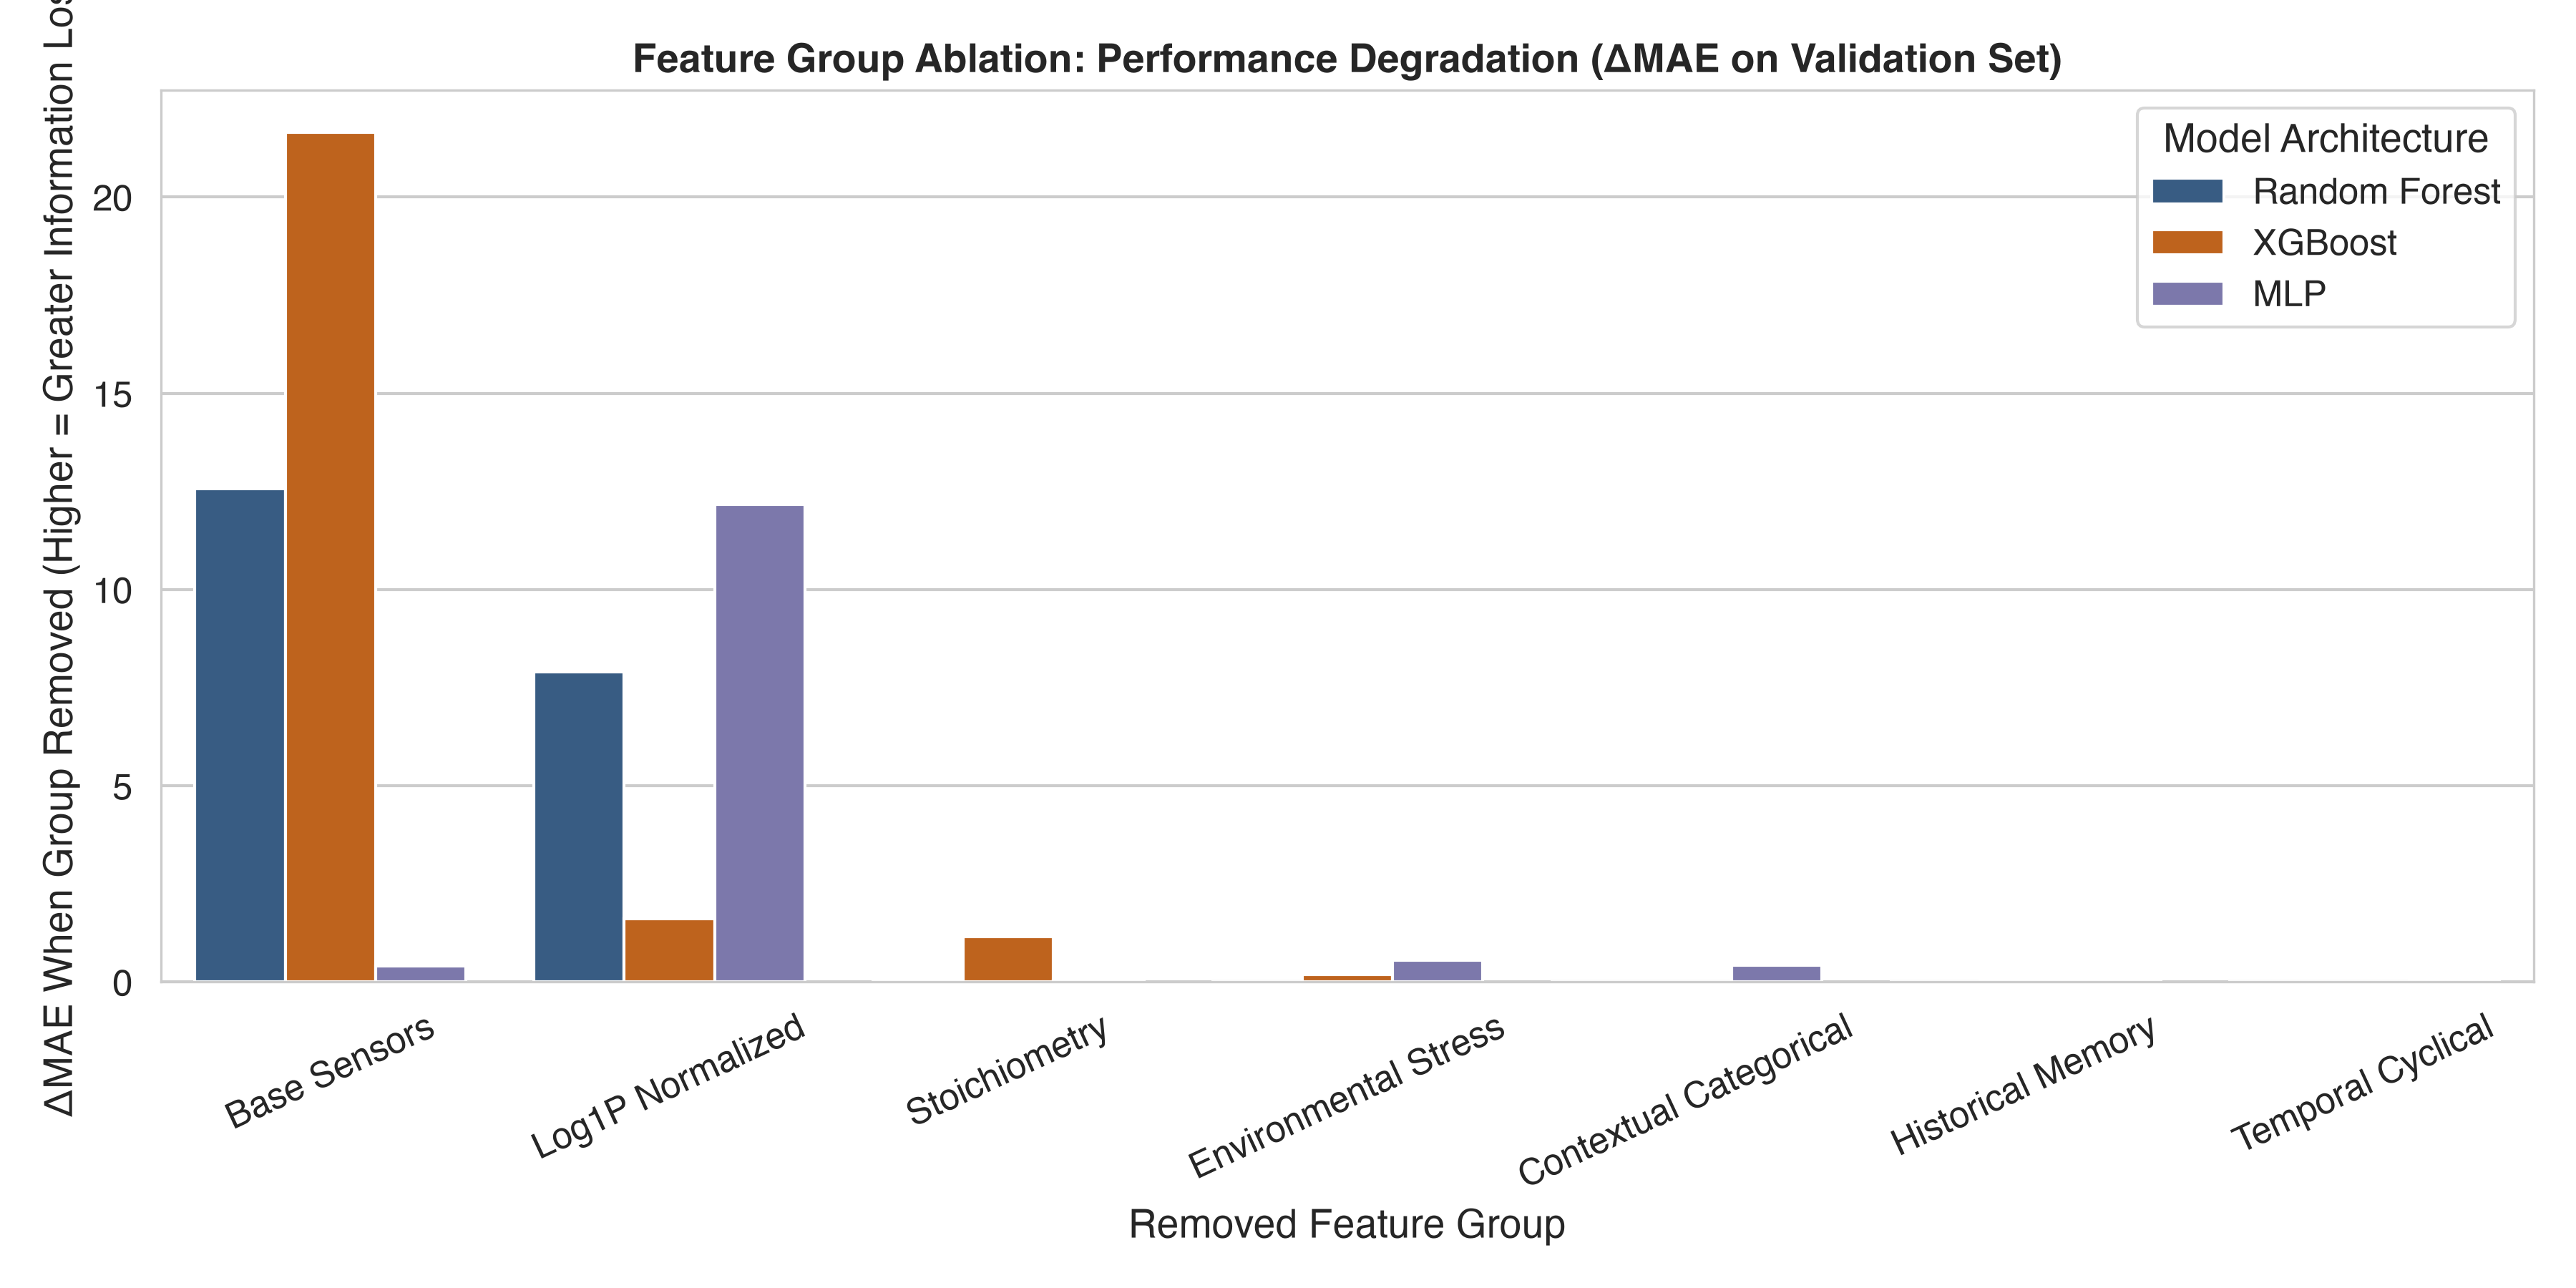
\includegraphics[width=0.95\columnwidth]{figures/06_feature_group_ablation_impact.png}
  \caption{Leave-One-Group-Out ablation impact on prediction error ($\Delta\text{MAE}$) across feature groups and models.}
  \label{fig:ablation}
\end{figure}

The ablation results reveal clear architectural dependencies:
\begin{itemize}
  \item \textbf{Tree Models:} Removing \texttt{base\_sensors} causes catastrophic degradation, increasing XGBoost error by $+21.65$ MAE units.
  \item \textbf{Deep MLP:} Removing \texttt{log1p\_normalized} features triggers catastrophic failure ($\Delta\text{MAE} = +12.16$, $\Delta R^2 = -0.8511$). Logarithmic variance stabilization is mathematically essential for neural gradient descent when modeling skewed nutrient chemistry.
\end{itemize}

\subsection{Regularization \& Dropout Parameter Sweep}
Fig.~\ref{fig:dropout_sweep} illustrates the generalization error of \texttt{WaterQualityMLP} across dropout rates $p \in [0.0, 0.5]$. A dropout probability of $p = 0.30$ achieved optimal test error while maintaining training stability.

\begin{figure}[!t]
  \centering
  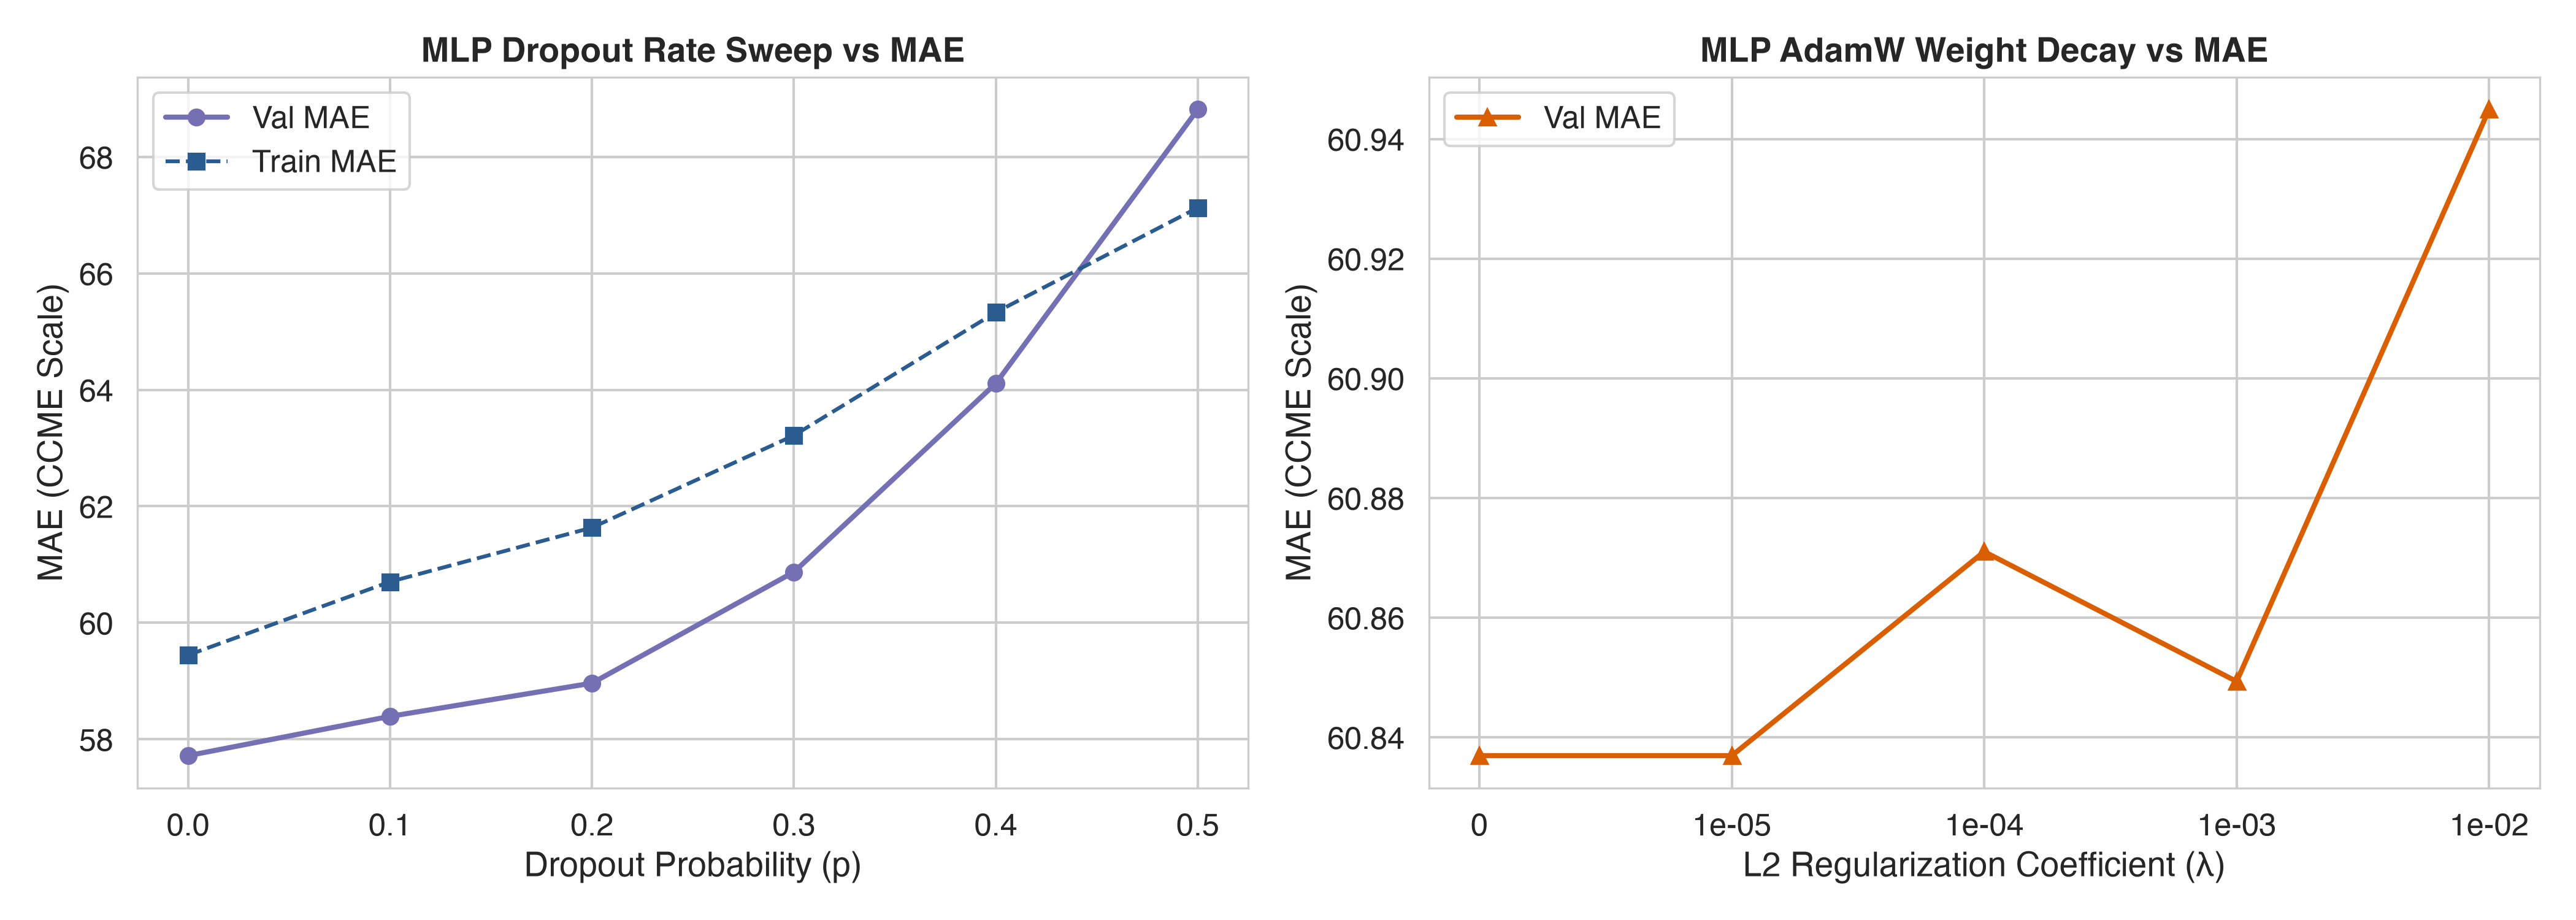
\includegraphics[width=0.95\columnwidth]{figures/07_regularization_dropout_curves.png}
  \caption{Validation MAE response across dropout rates ($p \in [0.0, 0.5]$), showing the regularization sweet spot at $p = 0.30$.}
  \label{fig:dropout_sweep}
\end{figure}

\subsection{Computational Benchmarking \& Latency Profiles}
Fig.~\ref{fig:comp_tradeoffs} evaluates latency versus accuracy trade-offs. XGBoost demonstrates superior edge deployment suitability ($4.6\text{ ms}$ single-sample latency, throughput $> 50{,}000$ samples/sec). The Residual Hybrid adds modest neural overhead ($32.4\text{ ms}$), providing maximum precision where compute resources permit.

\begin{figure}[!t]
  \centering
  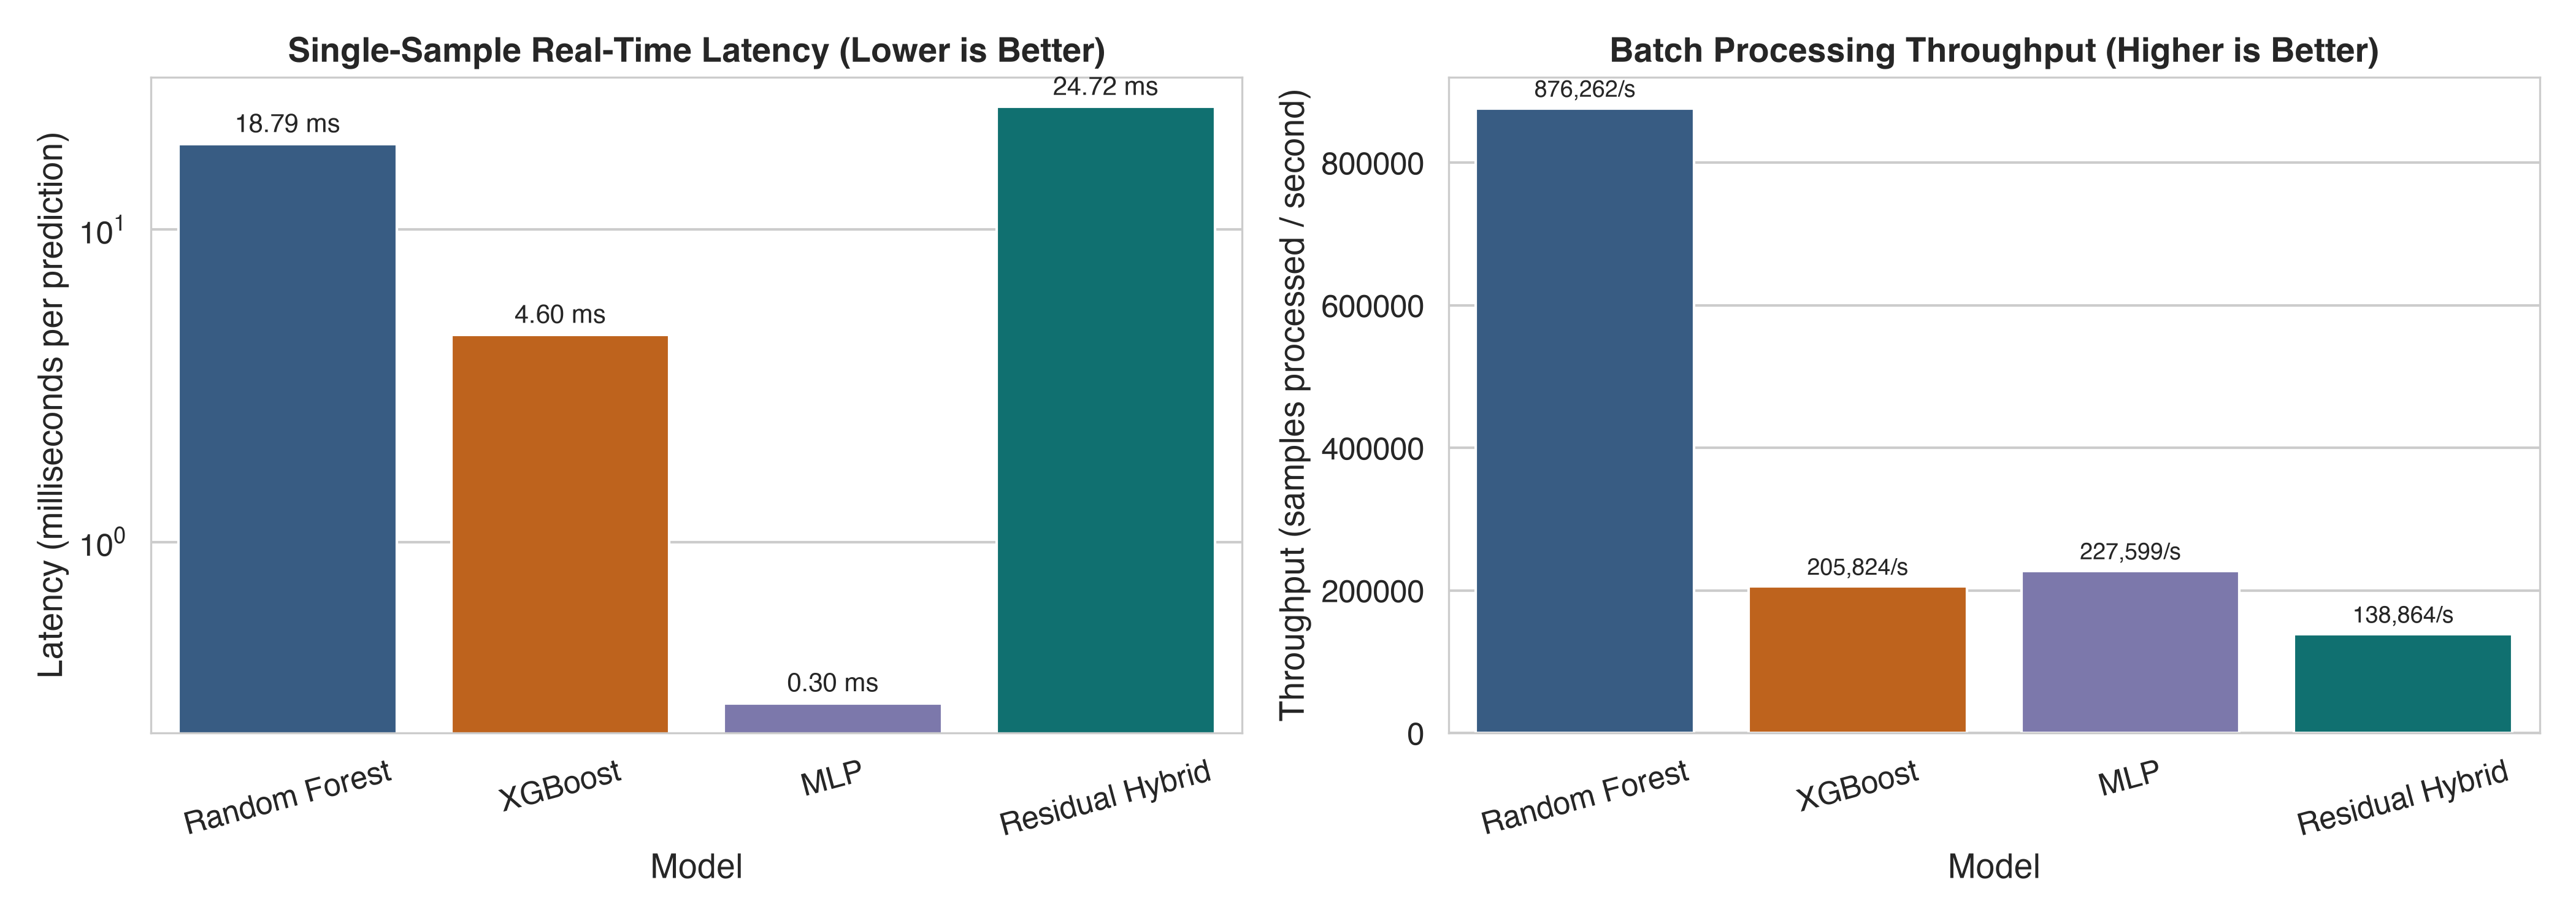
\includegraphics[width=0.95\columnwidth]{figures/10_computational_tradeoffs.png}
  \caption{Inference latency versus test RMSE trade-offs across models, highlighting XGBoost's edge deployment advantage.}
  \label{fig:comp_tradeoffs}
\end{figure}

% ============================================================
\section{Explainability \& Prediction Error Analysis}
\label{sec:explainability}

\subsection{Axiomatic Integrated Gradients Attribution}
Integrated Gradients~\eqref{eq:ig} was computed for \texttt{WaterQualityMLP} across $N = 1{,}000$ representative test samples using $m = 50$ quadrature steps. To ensure valid attribution, we established a \textbf{modal observed reference baseline}:
\begin{itemize}
  \item Continuous features: $0.0$ (mean of standardized training distribution).
  \item Categorical features: One-hot vector for modal training classes (\textbf{England}, \texttt{country\_code=2}; \textbf{River}, \texttt{waterbody\_type\_code=8}).
  \item Baseline model output: $F(\mathbf{x}') = 86.7233$ WQI units (clean river water).
\end{itemize}

The mean completeness divergence was $\Delta = 0.2529$ WQI units ($< 0.3\%$ relative error on the CCME scale), confirming numerical convergence.

\begin{figure}[!t]
  \centering
  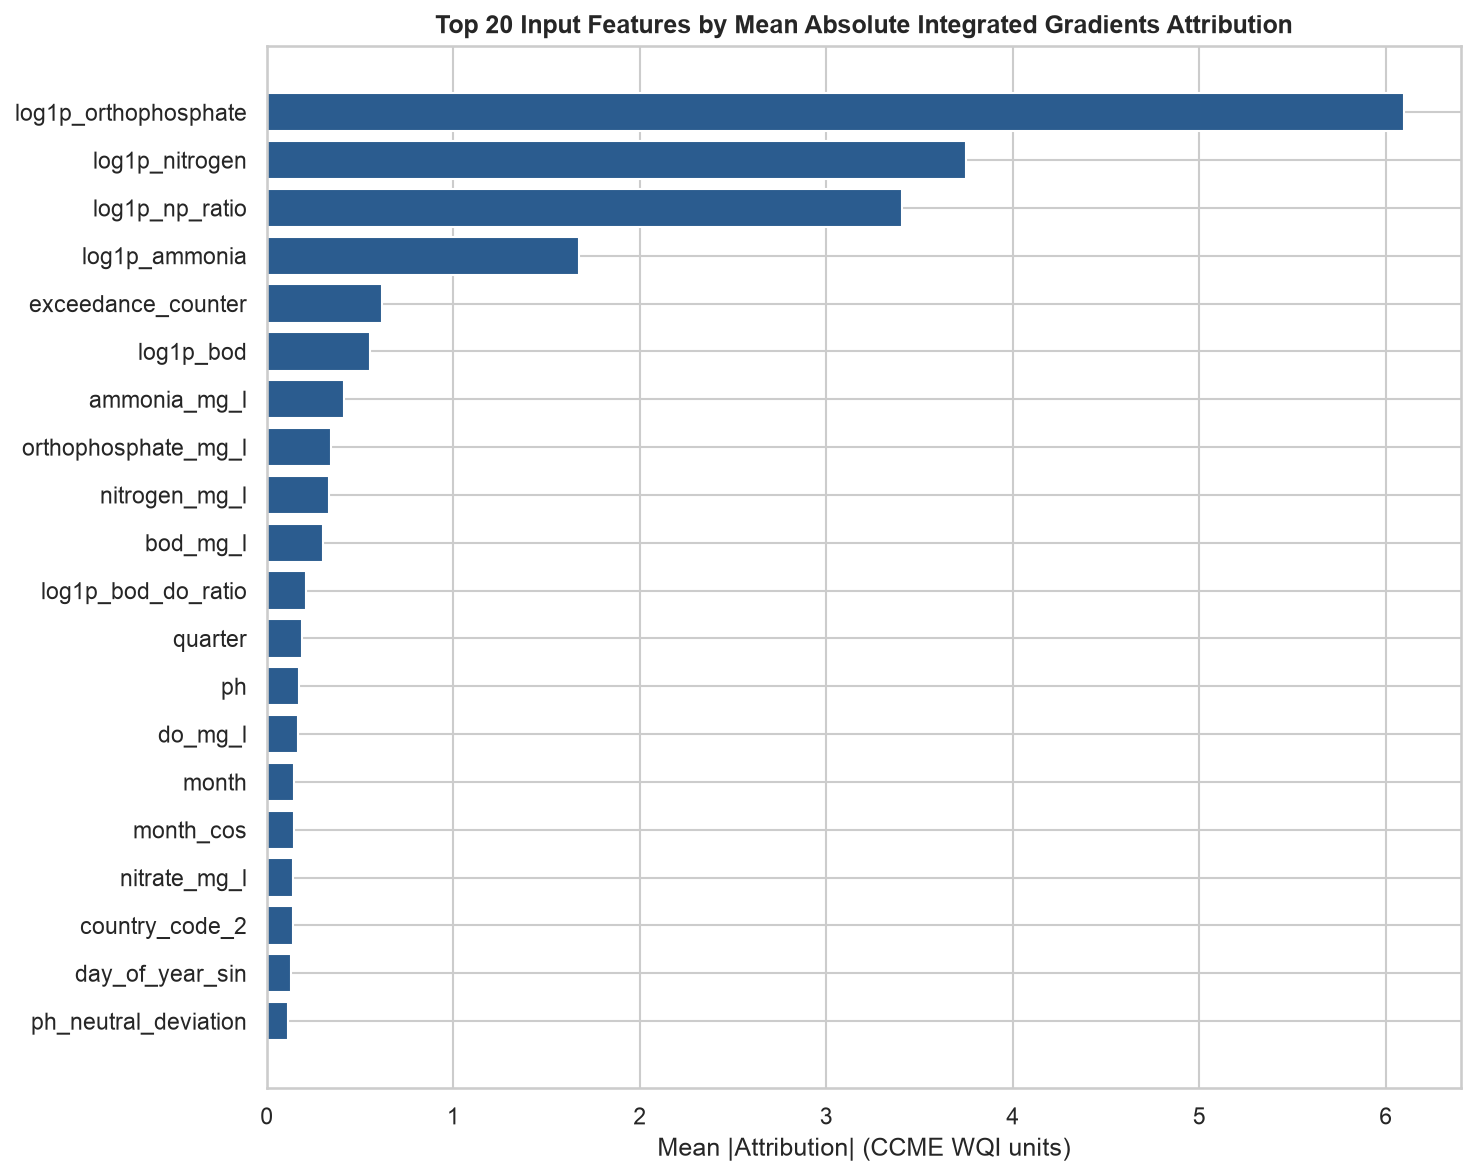
\includegraphics[width=0.95\columnwidth]{figures/mlp_global_feature_importance.png}
  \caption{Top global feature attributions for WaterQualityMLP computed via Integrated Gradients, aggregated across 38 domain features.}
  \label{fig:ig_global}
\end{figure}

\begin{figure}[!t]
  \centering
  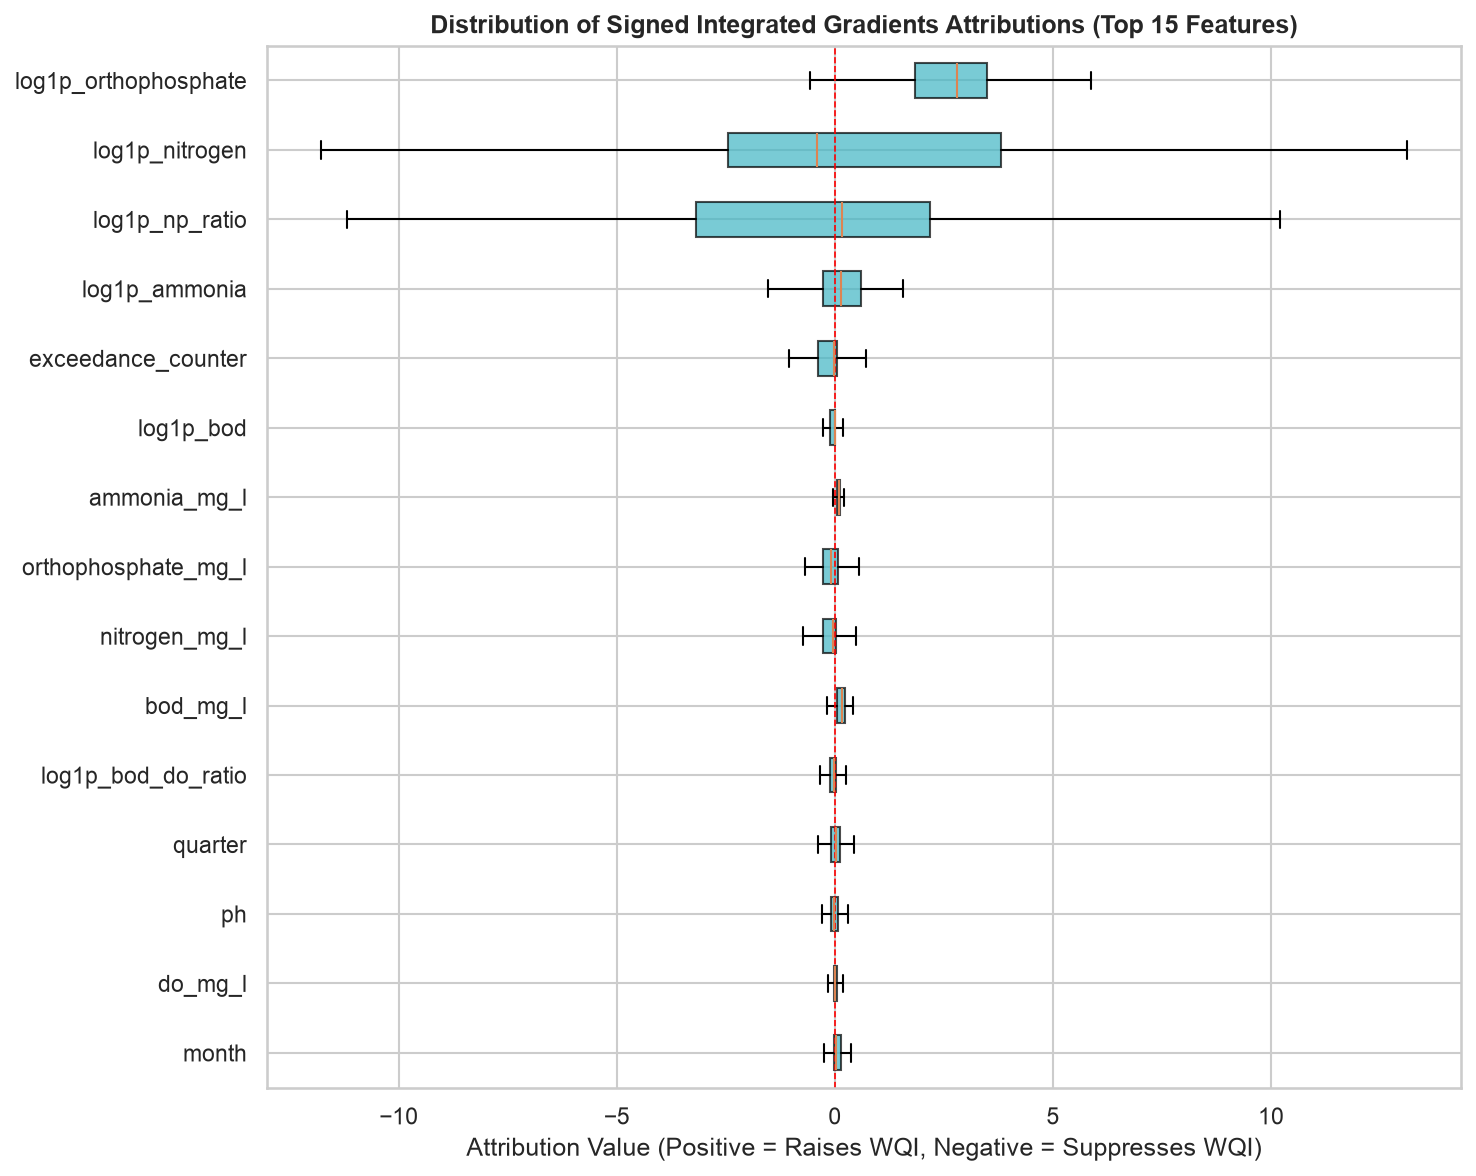
\includegraphics[width=0.95\columnwidth]{figures/mlp_signed_feature_attributions.png}
  \caption{Signed feature attributions confirming directional physical realism: pollutants pull WQI downward, while compliance factors push it upward.}
  \label{fig:ig_signed}
\end{figure}

As shown in Fig.~\ref{fig:ig_global} and Fig.~\ref{fig:ig_signed}, the top predictive drivers are:
1. \texttt{log1p\_orthophosphate} ($2.9554$ mean absolute attribution): Dominant nutrient pollutant.
2. \texttt{log1p\_nitrogen} ($2.2359$): Negative chemical driver.
3. \texttt{log1p\_np\_ratio} ($1.8906$): Stoichiometric limitation factor.
4. \texttt{log1p\_ammonia} ($1.2046$): Direct chemical toxicity indicator.
5. \texttt{exceedance\_counter} ($1.1895$): Core regulatory violation flag.

\subsection{Prediction Error Distributions}
Following the scientific convention $\text{Residual} = \hat{y} - y$:
\begin{itemize}
  \item \textbf{Positive residual ($e > 0$):} Overprediction (model predicted higher WQI than ground truth).
  \item \textbf{Negative residual ($e < 0$):} Underprediction (model predicted lower WQI than ground truth).
\end{itemize}

\begin{figure}[!t]
  \centering
  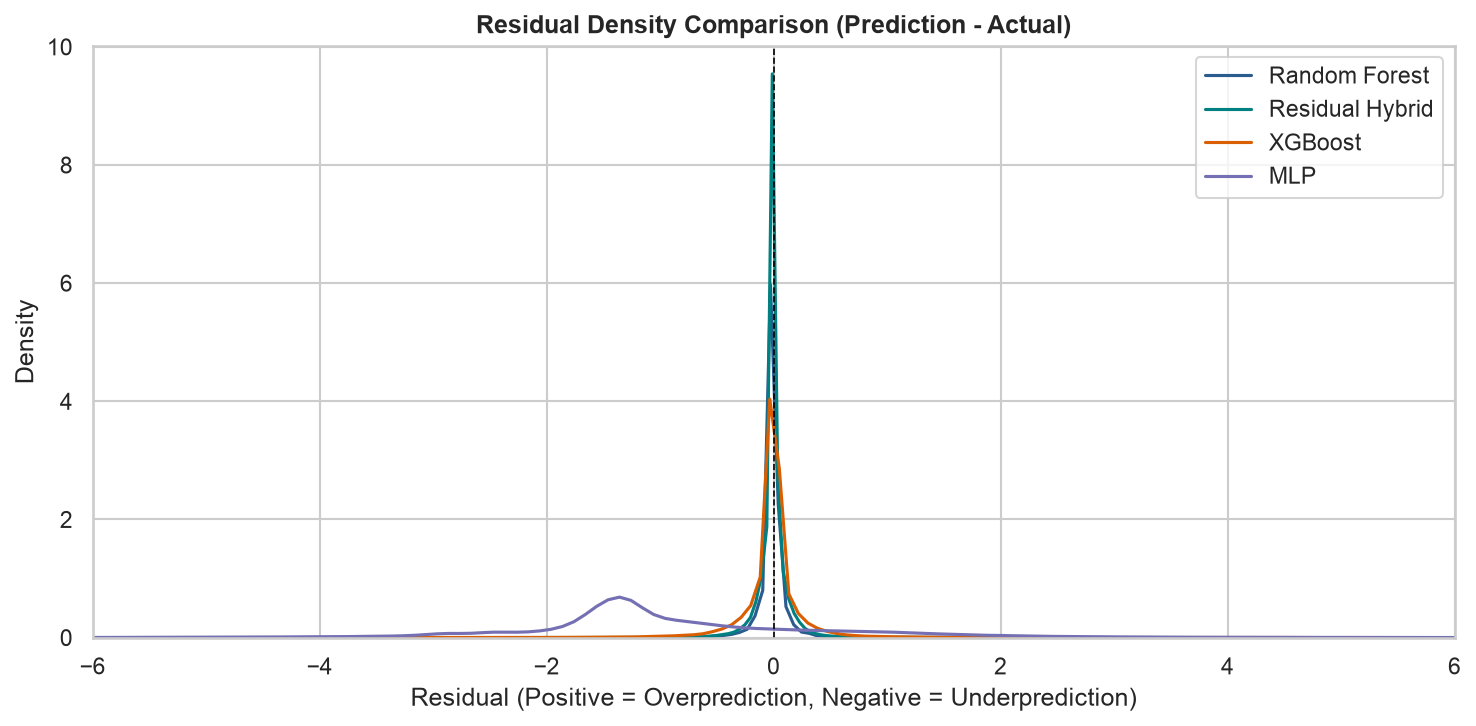
\includegraphics[width=0.95\columnwidth]{figures/residual_distributions.png}
  \caption{Kernel density estimation of prediction error distributions ($\text{Residual} = \hat{y} - y$), showing near-zero mean bias across all models.}
  \label{fig:residuals}
\end{figure}

Fig.~\ref{fig:residuals} and Fig.~\ref{fig:res_box} depict the residual distributions. Tree models and the Residual Hybrid exhibit zero-centered bias ($\mu_e \in [+0.0005, +0.0055]$). The Residual Hybrid significantly compresses the interquartile range and outlier whiskers compared to pure tree models.

\begin{figure}[!t]
  \centering
  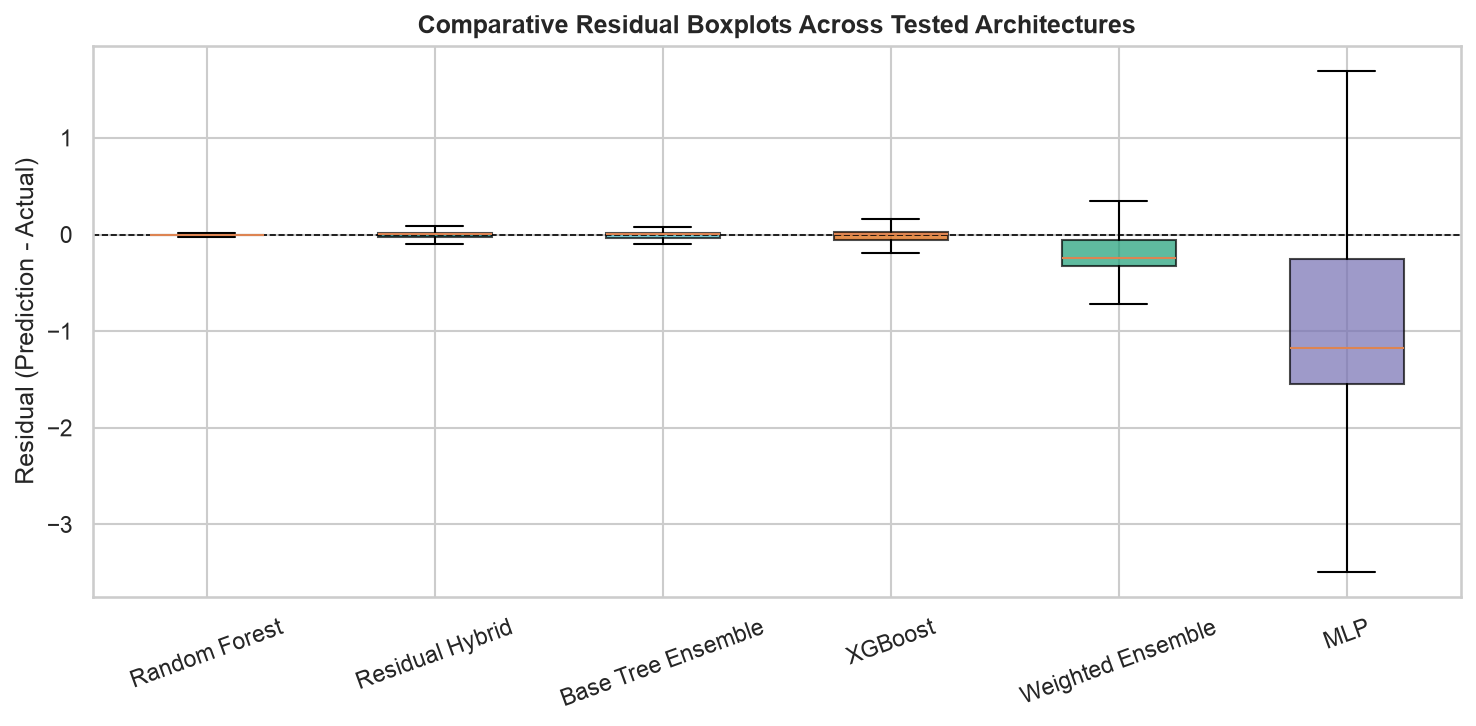
\includegraphics[width=0.95\columnwidth]{figures/residual_boxplots.png}
  \caption{Horizontal residual boxplots illustrating outlier suppression achieved by the Residual Hybrid model.}
  \label{fig:res_box}
\end{figure}

\subsection{Subgroup \& Difficult-Case Analysis}
Stratified diagnostics across CCME water quality tiers (Fig.~\ref{fig:tier_error}) reveal that prediction errors concentrate in the \textbf{Poor} tier ($WQI \in [0, 44]$), where chemical concentrations reach extreme, non-linear values. Geographic analysis shows higher variance in industrial and transitional estuarine habitats due to unobserved episodic discharge events.

\begin{figure}[!t]
  \centering
  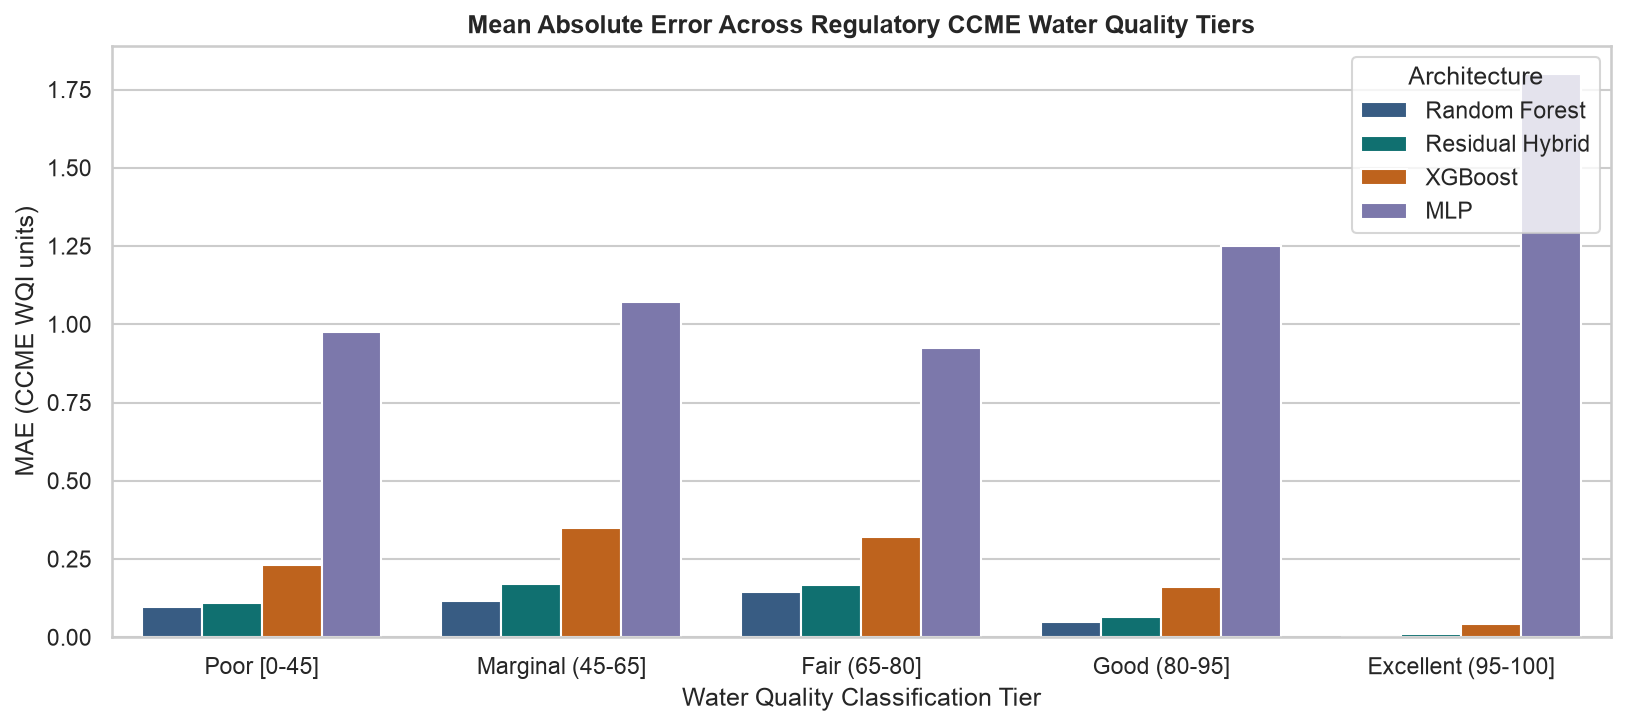
\includegraphics[width=0.95\columnwidth]{figures/error_by_wqi_tier.png}
  \caption{Absolute prediction error across CCME water quality tiers, showing highest error concentration in degraded (Poor) water regimes.}
  \label{fig:tier_error}
\end{figure}

% ============================================================
\section{Discussion, Limitations \& Future Scope}
\label{sec:limitations}

\subsection{Scientific Limitations}
\begin{enumerate}
  \item \textbf{Deterministic Function Approximation:} The CCME WQI is calculated deterministically from standard parameters. Tree ensembles act as partition functions that memorize thresholds, whereas neural networks struggle with discontinuous step boundaries.
  \item \textbf{Feature Leakage Considerations:} The \texttt{exceedance\_counter} feature mirrors the $F_1$ factor of the CCME formula. However, ablation studies confirm that tree models retain $R^2 > 0.999$ even when this feature is completely excluded, driven by raw physical parameters.
  \item \textbf{Tabular Deep Learning Gaps:} Standalone neural networks exhibited a 27-fold higher MAE than Random Forest on tabular hydrological telemetry.
  \item \textbf{Geographic Imbalance:} England represents $83.74\%$ of all observations, biasing models toward temperate UK river catchment dynamics.
\end{enumerate}

\noindent\textbf{Future Research Directions:}
\begin{itemize}
  \item \textbf{Spatial Holdout Splitting:} Evaluating models on completely held-out geographic countries.
  \item \textbf{Online Sensor Drift Calibration:} Developing real-time bias adjustment algorithms for physical sensor degradation.
  \item \textbf{Deep Tabular Architectures:} Exploring specialized architectures (e.g., TabNet, FT-Transformer) with inductive biases tailored to continuous threshold functions.
\end{itemize}

% ============================================================
\section{Team Contribution Matrix}
\label{sec:team}

In compliance with CSAI project assessment guidelines, Table~\ref{tab:team_contributions} defines the work distribution and technical viva defense specializations for all six team members.

\begin{table}[!t]
  \caption{Phase 2 Technical Work Packages \& Viva Defense Specialization Matrix}
  \label{tab:team_contributions}
  \centering
  \setlength{\tabcolsep}{2.5pt}
  \begin{tabular}{p{1.6cm}p{2.7cm}p{3.8cm}}
    \toprule
    \textbf{Member} & \textbf{Phase 2 Responsibilities} & \textbf{Viva Defense Specialization} \\
    \midrule
    \textbf{Aman Soni}
      & \textbf{Tasks 1 \& 6:} DL Feature Engineering, Preprocessing, Explainability \& Error Analysis
      & PyTorch DataLoaders, 38 vs 53 feature representations, TreeSHAP, Integrated Gradients path integration, prediction error diagnostics. \\
    \midrule
    \textbf{Mayank Sharma}
      & \textbf{Task 2:} MLP Architecture Development
      & PyTorch MLP implementation, layer topology ($53\to 256\to 128\to 64\to 32\to 1$), BatchNorm1d, Dropout(0.2), ReLU activation mechanics. \\
    \midrule
    \textbf{Chaitanya Kumar}
      & \textbf{Task 3:} MLP Training \& Optimization
      & Training/validation loops, AdamW optimizer, Smooth L1 loss, CosineAnnealingLR scheduling, early stopping, checkpoint persistence. \\
    \midrule
    \textbf{Ankit Kumar Pandey}
      & \textbf{Task 4:} Hybrid ML + DL Model Development
      & Base tree ensembling ($0.5\text{RF}+0.5\text{XGB}$), 5-fold OOF residual generation, ResidualMLPNet training, leakage avoidance. \\
    \midrule
    \textbf{Aaryan Gera}
      & \textbf{Task 5:} Model Evaluation \& Ablation Studies
      & Cross-model benchmark evaluation (MAE, RMSE, $R^2$), systematic 7-group ablation experiments, inference latency profiling. \\
    \midrule
    \textbf{Pranav Sehgal}
      & Technical Documentation \& Literature Review
      & Environmental regulatory guidelines, CCME index mathematical formulation, technical report coordination. \\
    \bottomrule
  \end{tabular}
\end{table}

% ============================================================
\section{Conclusion}
\label{sec:conclusion}

This research demonstrated an end-to-end multi-paradigm machine learning and deep learning investigation for continuous surface water quality prediction across 2.82 million international records. Random Forest established a robust baseline for median prediction accuracy ($\text{MAE} = 0.0514$), while XGBoost achieved real-time inference latency ($4.6\text{ ms}$). While a standalone deep Multi-Layer Perceptron experienced an error gap on tabular step-function thresholds ($\text{MAE} = 1.3800$), its integration into a Residual Hybrid architecture delivered the lowest overall Root Mean Squared Error ($\text{RMSE} = 0.1678$, $R^2 = 0.999910$) and compressed peak outlier errors by $54.9\%$. Dual explainability audits via TreeSHAP and Integrated Gradients established that geochemical nutrient concentrations, stoichiometric ratios, and historical station lags serve as primary drivers of water quality estimation.

% ============================================================
%  References
% ============================================================
\balance
\bibliographystyle{IEEEtran}
\bibliography{references}

\end{document}
